\documentclass[twoside]{book}

% Packages required by doxygen
\usepackage{fixltx2e}
\usepackage{calc}
\usepackage{doxygen}
\usepackage[export]{adjustbox} % also loads graphicx
\usepackage{graphicx}
\usepackage[utf8]{inputenc}
\usepackage{makeidx}
\usepackage{multicol}
\usepackage{multirow}
\PassOptionsToPackage{warn}{textcomp}
\usepackage{textcomp}
\usepackage[nointegrals]{wasysym}
\usepackage[table]{xcolor}

% Font selection
\usepackage[T1]{fontenc}
\usepackage[scaled=.90]{helvet}
\usepackage{courier}
\usepackage{amssymb}
\usepackage{sectsty}
\renewcommand{\familydefault}{\sfdefault}
\allsectionsfont{%
  \fontseries{bc}\selectfont%
  \color{darkgray}%
}
\renewcommand{\DoxyLabelFont}{%
  \fontseries{bc}\selectfont%
  \color{darkgray}%
}
\newcommand{\+}{\discretionary{\mbox{\scriptsize$\hookleftarrow$}}{}{}}

% Page & text layout
\usepackage{geometry}
\geometry{%
  a4paper,%
  top=2.5cm,%
  bottom=2.5cm,%
  left=2.5cm,%
  right=2.5cm%
}
\tolerance=750
\hfuzz=15pt
\hbadness=750
\setlength{\emergencystretch}{15pt}
\setlength{\parindent}{0cm}
\setlength{\parskip}{3ex plus 2ex minus 2ex}
\makeatletter
\renewcommand{\paragraph}{%
  \@startsection{paragraph}{4}{0ex}{-1.0ex}{1.0ex}{%
    \normalfont\normalsize\bfseries\SS@parafont%
  }%
}
\renewcommand{\subparagraph}{%
  \@startsection{subparagraph}{5}{0ex}{-1.0ex}{1.0ex}{%
    \normalfont\normalsize\bfseries\SS@subparafont%
  }%
}
\makeatother

% Headers & footers
\usepackage{fancyhdr}
\pagestyle{fancyplain}
\fancyhead[LE]{\fancyplain{}{\bfseries\thepage}}
\fancyhead[CE]{\fancyplain{}{}}
\fancyhead[RE]{\fancyplain{}{\bfseries\leftmark}}
\fancyhead[LO]{\fancyplain{}{\bfseries\rightmark}}
\fancyhead[CO]{\fancyplain{}{}}
\fancyhead[RO]{\fancyplain{}{\bfseries\thepage}}
\fancyfoot[LE]{\fancyplain{}{}}
\fancyfoot[CE]{\fancyplain{}{}}
\fancyfoot[RE]{\fancyplain{}{\bfseries\scriptsize Generated by Doxygen }}
\fancyfoot[LO]{\fancyplain{}{\bfseries\scriptsize Generated by Doxygen }}
\fancyfoot[CO]{\fancyplain{}{}}
\fancyfoot[RO]{\fancyplain{}{}}
\renewcommand{\footrulewidth}{0.4pt}
\renewcommand{\chaptermark}[1]{%
  \markboth{#1}{}%
}
\renewcommand{\sectionmark}[1]{%
  \markright{\thesection\ #1}%
}

% Indices & bibliography
\usepackage{natbib}
\usepackage[titles]{tocloft}
\setcounter{tocdepth}{3}
\setcounter{secnumdepth}{5}
\makeindex

% Hyperlinks (required, but should be loaded last)
\usepackage{ifpdf}
\ifpdf
  \usepackage[pdftex,pagebackref=true]{hyperref}
\else
  \usepackage[ps2pdf,pagebackref=true]{hyperref}
\fi
\hypersetup{%
  colorlinks=true,%
  linkcolor=blue,%
  citecolor=blue,%
  unicode%
}

% Custom commands
\newcommand{\clearemptydoublepage}{%
  \newpage{\pagestyle{empty}\cleardoublepage}%
}

\usepackage{caption}
\captionsetup{labelsep=space,justification=centering,font={bf},singlelinecheck=off,skip=4pt,position=top}

%===== C O N T E N T S =====

\begin{document}

% Titlepage & ToC
\hypersetup{pageanchor=false,
             bookmarksnumbered=true,
             pdfencoding=unicode
            }
\pagenumbering{alph}
\begin{titlepage}
\vspace*{7cm}
\begin{center}%
{\Large Bank\+App }\\
\vspace*{1cm}
{\large Generated by Doxygen 1.8.13}\\
\end{center}
\end{titlepage}
\clearemptydoublepage
\pagenumbering{roman}
\tableofcontents
\clearemptydoublepage
\pagenumbering{arabic}
\hypersetup{pageanchor=true}

%--- Begin generated contents ---
\chapter{Namespace Index}
\section{Packages}
Here are the packages with brief descriptions (if available)\+:\begin{DoxyCompactList}
\item\contentsline{section}{\hyperlink{namespacebankapp}{bankapp} }{\pageref{namespacebankapp}}{}
\item\contentsline{section}{\hyperlink{namespacebankapp_1_1client}{bankapp.\+client} }{\pageref{namespacebankapp_1_1client}}{}
\item\contentsline{section}{\hyperlink{namespacebankapp_1_1server}{bankapp.\+server} }{\pageref{namespacebankapp_1_1server}}{}
\end{DoxyCompactList}

\chapter{Hierarchical Index}
\section{Class Hierarchy}
This inheritance list is sorted roughly, but not completely, alphabetically\+:\begin{DoxyCompactList}
\item \contentsline{section}{bankapp.\+server.\+Account}{\pageref{classbankapp_1_1server_1_1_account}}{}
\begin{DoxyCompactList}
\item \contentsline{section}{bankapp.\+server.\+Admin}{\pageref{classbankapp_1_1server_1_1_admin}}{}
\item \contentsline{section}{bankapp.\+server.\+User}{\pageref{classbankapp_1_1server_1_1_user}}{}
\end{DoxyCompactList}
\item \contentsline{section}{bankapp.\+server.\+bank\+Account}{\pageref{classbankapp_1_1server_1_1bank_account}}{}
\item \contentsline{section}{bankapp.\+server.\+bank\+Account\+Test}{\pageref{classbankapp_1_1server_1_1bank_account_test}}{}
\item \contentsline{section}{bankapp.\+client.\+bank\+Client}{\pageref{classbankapp_1_1client_1_1bank_client}}{}
\item \contentsline{section}{bankapp.\+client.\+bank\+Controller}{\pageref{classbankapp_1_1client_1_1bank_controller}}{}
\item \contentsline{section}{bankapp.\+server.\+bank\+Server}{\pageref{classbankapp_1_1server_1_1bank_server}}{}
\item \contentsline{section}{bankapp.\+server.\+B\+D\+Test}{\pageref{classbankapp_1_1server_1_1_b_d_test}}{}
\item \contentsline{section}{bankapp.\+server.\+Ibank\+D\+AO}{\pageref{interfacebankapp_1_1server_1_1_ibank_d_a_o}}{}
\begin{DoxyCompactList}
\item \contentsline{section}{bankapp.\+server.\+bank\+D\+AO}{\pageref{classbankapp_1_1server_1_1bank_d_a_o}}{}
\end{DoxyCompactList}
\item \contentsline{section}{bankapp.\+server.\+Performance}{\pageref{classbankapp_1_1server_1_1_performance}}{}
\item \contentsline{section}{bankapp.\+server.\+Report}{\pageref{classbankapp_1_1server_1_1_report}}{}
\item \contentsline{section}{bankapp.\+server.\+Report\+Test}{\pageref{classbankapp_1_1server_1_1_report_test}}{}
\item \contentsline{section}{bankapp.\+client.\+R\+M\+I\+Service\+Locator}{\pageref{classbankapp_1_1client_1_1_r_m_i_service_locator}}{}
\item \contentsline{section}{bankapp.\+server.\+Server\+Test}{\pageref{classbankapp_1_1server_1_1_server_test}}{}
\item \contentsline{section}{bankapp.\+server.\+User\+Test}{\pageref{classbankapp_1_1server_1_1_user_test}}{}
\item Remote\begin{DoxyCompactList}
\item \contentsline{section}{bankapp.\+server.\+I\+B\+Manager}{\pageref{interfacebankapp_1_1server_1_1_i_b_manager}}{}
\begin{DoxyCompactList}
\item \contentsline{section}{bankapp.\+server.\+B\+Manager}{\pageref{classbankapp_1_1server_1_1_b_manager}}{}
\end{DoxyCompactList}
\end{DoxyCompactList}
\item Unicast\+Remote\+Object\begin{DoxyCompactList}
\item \contentsline{section}{bankapp.\+server.\+B\+Manager}{\pageref{classbankapp_1_1server_1_1_b_manager}}{}
\end{DoxyCompactList}
\end{DoxyCompactList}

\chapter{Class Index}
\section{Class List}
Here are the classes, structs, unions and interfaces with brief descriptions\+:\begin{DoxyCompactList}
\item\contentsline{section}{\hyperlink{classbankapp_1_1server_1_1_account}{bankapp.\+server.\+Account} }{\pageref{classbankapp_1_1server_1_1_account}}{}
\item\contentsline{section}{\hyperlink{classbankapp_1_1server_1_1_admin}{bankapp.\+server.\+Admin} }{\pageref{classbankapp_1_1server_1_1_admin}}{}
\item\contentsline{section}{\hyperlink{classbankapp_1_1server_1_1bank_account}{bankapp.\+server.\+bank\+Account} }{\pageref{classbankapp_1_1server_1_1bank_account}}{}
\item\contentsline{section}{\hyperlink{classbankapp_1_1server_1_1bank_account_test}{bankapp.\+server.\+bank\+Account\+Test} }{\pageref{classbankapp_1_1server_1_1bank_account_test}}{}
\item\contentsline{section}{\hyperlink{classbankapp_1_1client_1_1bank_client}{bankapp.\+client.\+bank\+Client} }{\pageref{classbankapp_1_1client_1_1bank_client}}{}
\item\contentsline{section}{\hyperlink{classbankapp_1_1client_1_1bank_controller}{bankapp.\+client.\+bank\+Controller} }{\pageref{classbankapp_1_1client_1_1bank_controller}}{}
\item\contentsline{section}{\hyperlink{classbankapp_1_1server_1_1bank_d_a_o}{bankapp.\+server.\+bank\+D\+AO} }{\pageref{classbankapp_1_1server_1_1bank_d_a_o}}{}
\item\contentsline{section}{\hyperlink{classbankapp_1_1server_1_1bank_server}{bankapp.\+server.\+bank\+Server} }{\pageref{classbankapp_1_1server_1_1bank_server}}{}
\item\contentsline{section}{\hyperlink{classbankapp_1_1server_1_1_b_d_test}{bankapp.\+server.\+B\+D\+Test} }{\pageref{classbankapp_1_1server_1_1_b_d_test}}{}
\item\contentsline{section}{\hyperlink{classbankapp_1_1server_1_1_b_manager}{bankapp.\+server.\+B\+Manager} }{\pageref{classbankapp_1_1server_1_1_b_manager}}{}
\item\contentsline{section}{\hyperlink{interfacebankapp_1_1server_1_1_ibank_d_a_o}{bankapp.\+server.\+Ibank\+D\+AO} }{\pageref{interfacebankapp_1_1server_1_1_ibank_d_a_o}}{}
\item\contentsline{section}{\hyperlink{interfacebankapp_1_1server_1_1_i_b_manager}{bankapp.\+server.\+I\+B\+Manager} }{\pageref{interfacebankapp_1_1server_1_1_i_b_manager}}{}
\item\contentsline{section}{\hyperlink{classbankapp_1_1server_1_1_performance}{bankapp.\+server.\+Performance} }{\pageref{classbankapp_1_1server_1_1_performance}}{}
\item\contentsline{section}{\hyperlink{classbankapp_1_1server_1_1_report}{bankapp.\+server.\+Report} }{\pageref{classbankapp_1_1server_1_1_report}}{}
\item\contentsline{section}{\hyperlink{classbankapp_1_1server_1_1_report_test}{bankapp.\+server.\+Report\+Test} }{\pageref{classbankapp_1_1server_1_1_report_test}}{}
\item\contentsline{section}{\hyperlink{classbankapp_1_1client_1_1_r_m_i_service_locator}{bankapp.\+client.\+R\+M\+I\+Service\+Locator} }{\pageref{classbankapp_1_1client_1_1_r_m_i_service_locator}}{}
\item\contentsline{section}{\hyperlink{classbankapp_1_1server_1_1_server_test}{bankapp.\+server.\+Server\+Test} }{\pageref{classbankapp_1_1server_1_1_server_test}}{}
\item\contentsline{section}{\hyperlink{classbankapp_1_1server_1_1_user}{bankapp.\+server.\+User} }{\pageref{classbankapp_1_1server_1_1_user}}{}
\item\contentsline{section}{\hyperlink{classbankapp_1_1server_1_1_user_test}{bankapp.\+server.\+User\+Test} }{\pageref{classbankapp_1_1server_1_1_user_test}}{}
\end{DoxyCompactList}

\chapter{File Index}
\section{File List}
Here is a list of all files with brief descriptions\+:\begin{DoxyCompactList}
\item\contentsline{section}{src/main/java/bankapp/client/\hyperlink{_bank_client_8java}{Bank\+Client.\+java} }{\pageref{_bank_client_8java}}{}
\item\contentsline{section}{src/main/java/bankapp/client/\hyperlink{_bank_controller_8java}{Bank\+Controller.\+java} }{\pageref{_bank_controller_8java}}{}
\item\contentsline{section}{src/main/java/bankapp/client/\hyperlink{_r_m_i_service_locator_8java}{R\+M\+I\+Service\+Locator.\+java} }{\pageref{_r_m_i_service_locator_8java}}{}
\item\contentsline{section}{src/main/java/bankapp/server/\hyperlink{_account_8java}{Account.\+java} }{\pageref{_account_8java}}{}
\item\contentsline{section}{src/main/java/bankapp/server/\hyperlink{_admin_8java}{Admin.\+java} }{\pageref{_admin_8java}}{}
\item\contentsline{section}{src/main/java/bankapp/server/\hyperlink{bank_account_8java}{bank\+Account.\+java} }{\pageref{bank_account_8java}}{}
\item\contentsline{section}{src/main/java/bankapp/server/\hyperlink{_bank_d_a_o_8java}{Bank\+D\+A\+O.\+java} }{\pageref{_bank_d_a_o_8java}}{}
\item\contentsline{section}{src/main/java/bankapp/server/\hyperlink{_bank_server_8java}{Bank\+Server.\+java} }{\pageref{_bank_server_8java}}{}
\item\contentsline{section}{src/main/java/bankapp/server/\hyperlink{_b_manager_8java}{B\+Manager.\+java} }{\pageref{_b_manager_8java}}{}
\item\contentsline{section}{src/main/java/bankapp/server/\hyperlink{_i_bank_d_a_o_8java}{I\+Bank\+D\+A\+O.\+java} }{\pageref{_i_bank_d_a_o_8java}}{}
\item\contentsline{section}{src/main/java/bankapp/server/\hyperlink{_i_b_manager_8java}{I\+B\+Manager.\+java} }{\pageref{_i_b_manager_8java}}{}
\item\contentsline{section}{src/main/java/bankapp/server/\hyperlink{_report_8java}{Report.\+java} }{\pageref{_report_8java}}{}
\item\contentsline{section}{src/main/java/bankapp/server/\hyperlink{_user_8java}{User.\+java} }{\pageref{_user_8java}}{}
\item\contentsline{section}{src/test/java/bankapp/server/\hyperlink{bank_account_test_8java}{bank\+Account\+Test.\+java} }{\pageref{bank_account_test_8java}}{}
\item\contentsline{section}{src/test/java/bankapp/server/\hyperlink{_b_d_test_8java}{B\+D\+Test.\+java} }{\pageref{_b_d_test_8java}}{}
\item\contentsline{section}{src/test/java/bankapp/server/\hyperlink{_performance_8java}{Performance.\+java} }{\pageref{_performance_8java}}{}
\item\contentsline{section}{src/test/java/bankapp/server/\hyperlink{_report_test_8java}{Report\+Test.\+java} }{\pageref{_report_test_8java}}{}
\item\contentsline{section}{src/test/java/bankapp/server/\hyperlink{_server_test_8java}{Server\+Test.\+java} }{\pageref{_server_test_8java}}{}
\item\contentsline{section}{src/test/java/bankapp/server/\hyperlink{_user_test_8java}{User\+Test.\+java} }{\pageref{_user_test_8java}}{}
\end{DoxyCompactList}

\chapter{Namespace Documentation}
\hypertarget{namespacebankapp}{}\section{Package bankapp}
\label{namespacebankapp}\index{bankapp@{bankapp}}
\subsection*{Packages}
\begin{DoxyCompactItemize}
\item 
package \hyperlink{namespacebankapp_1_1client}{client}
\item 
package \hyperlink{namespacebankapp_1_1server}{server}
\end{DoxyCompactItemize}

\hypertarget{namespacebankapp_1_1client}{}\section{Package bankapp.\+client}
\label{namespacebankapp_1_1client}\index{bankapp.\+client@{bankapp.\+client}}
\subsection*{Classes}
\begin{DoxyCompactItemize}
\item 
class \hyperlink{classbankapp_1_1client_1_1bank_client}{bank\+Client}
\item 
class \hyperlink{classbankapp_1_1client_1_1bank_controller}{bank\+Controller}
\item 
class \hyperlink{classbankapp_1_1client_1_1_r_m_i_service_locator}{R\+M\+I\+Service\+Locator}
\end{DoxyCompactItemize}

\hypertarget{namespacebankapp_1_1server}{}\section{Package bankapp.\+server}
\label{namespacebankapp_1_1server}\index{bankapp.\+server@{bankapp.\+server}}
\subsection*{Classes}
\begin{DoxyCompactItemize}
\item 
class \hyperlink{classbankapp_1_1server_1_1_account}{Account}
\item 
class \hyperlink{classbankapp_1_1server_1_1_admin}{Admin}
\item 
class \hyperlink{classbankapp_1_1server_1_1bank_account}{bank\+Account}
\item 
class \hyperlink{classbankapp_1_1server_1_1bank_account_test}{bank\+Account\+Test}
\item 
class \hyperlink{classbankapp_1_1server_1_1bank_d_a_o}{bank\+D\+AO}
\item 
class \hyperlink{classbankapp_1_1server_1_1bank_server}{bank\+Server}
\item 
class \hyperlink{classbankapp_1_1server_1_1_b_d_test}{B\+D\+Test}
\item 
class \hyperlink{classbankapp_1_1server_1_1_b_manager}{B\+Manager}
\item 
interface \hyperlink{interfacebankapp_1_1server_1_1_ibank_d_a_o}{Ibank\+D\+AO}
\item 
interface \hyperlink{interfacebankapp_1_1server_1_1_i_b_manager}{I\+B\+Manager}
\item 
class \hyperlink{classbankapp_1_1server_1_1_performance}{Performance}
\item 
class \hyperlink{classbankapp_1_1server_1_1_report}{Report}
\item 
class \hyperlink{classbankapp_1_1server_1_1_report_test}{Report\+Test}
\item 
class \hyperlink{classbankapp_1_1server_1_1_server_test}{Server\+Test}
\item 
class \hyperlink{classbankapp_1_1server_1_1_user}{User}
\item 
class \hyperlink{classbankapp_1_1server_1_1_user_test}{User\+Test}
\end{DoxyCompactItemize}

\chapter{Class Documentation}
\hypertarget{classbankapp_1_1server_1_1_account}{}\section{bankapp.\+server.\+Account Class Reference}
\label{classbankapp_1_1server_1_1_account}\index{bankapp.\+server.\+Account@{bankapp.\+server.\+Account}}
Inheritance diagram for bankapp.\+server.\+Account\+:\begin{figure}[H]
\begin{center}
\leavevmode
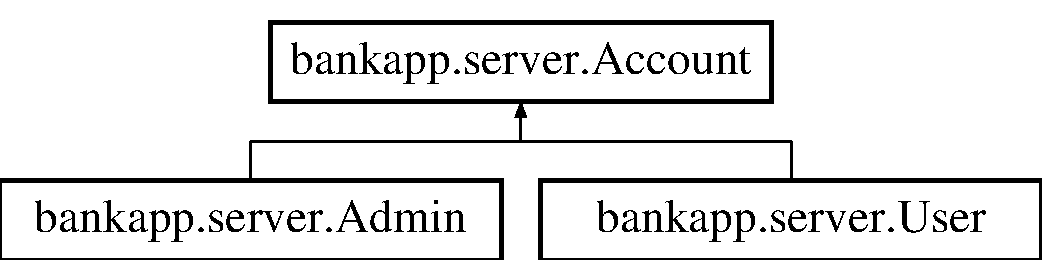
\includegraphics[height=2.000000cm]{classbankapp_1_1server_1_1_account}
\end{center}
\end{figure}
\subsection*{Public Member Functions}
\begin{DoxyCompactItemize}
\item 
\hyperlink{classbankapp_1_1server_1_1_account_a778b65b96a332ab3f7b2b2ad7da626a9}{Account} (String username, String pass)
\item 
String \hyperlink{classbankapp_1_1server_1_1_account_af1680fd62898dcc86a2e76c1f326f7d0}{get\+Username} ()
\item 
String \hyperlink{classbankapp_1_1server_1_1_account_a10506c227d9d68f13bc1b177c86c6da0}{get\+Pass} ()
\item 
void \hyperlink{classbankapp_1_1server_1_1_account_ab6a8bbb30450a1090fa9ee8770b25148}{set\+Pass} (String pass)
\item 
String \hyperlink{classbankapp_1_1server_1_1_account_af9ce01fe2afb9e196b9ea0ceb51eb3ae}{to\+String} ()
\end{DoxyCompactItemize}


\subsection{Detailed Description}


Definition at line 9 of file Account.\+java.



\subsection{Constructor \& Destructor Documentation}
\mbox{\Hypertarget{classbankapp_1_1server_1_1_account_a778b65b96a332ab3f7b2b2ad7da626a9}\label{classbankapp_1_1server_1_1_account_a778b65b96a332ab3f7b2b2ad7da626a9}} 
\index{bankapp\+::server\+::\+Account@{bankapp\+::server\+::\+Account}!Account@{Account}}
\index{Account@{Account}!bankapp\+::server\+::\+Account@{bankapp\+::server\+::\+Account}}
\subsubsection{\texorpdfstring{Account()}{Account()}}
{\footnotesize\ttfamily bankapp.\+server.\+Account.\+Account (\begin{DoxyParamCaption}\item[{String}]{username,  }\item[{String}]{pass }\end{DoxyParamCaption})}



Definition at line 13 of file Account.\+java.



\subsection{Member Function Documentation}
\mbox{\Hypertarget{classbankapp_1_1server_1_1_account_a10506c227d9d68f13bc1b177c86c6da0}\label{classbankapp_1_1server_1_1_account_a10506c227d9d68f13bc1b177c86c6da0}} 
\index{bankapp\+::server\+::\+Account@{bankapp\+::server\+::\+Account}!get\+Pass@{get\+Pass}}
\index{get\+Pass@{get\+Pass}!bankapp\+::server\+::\+Account@{bankapp\+::server\+::\+Account}}
\subsubsection{\texorpdfstring{get\+Pass()}{getPass()}}
{\footnotesize\ttfamily String bankapp.\+server.\+Account.\+get\+Pass (\begin{DoxyParamCaption}{ }\end{DoxyParamCaption})}



Definition at line 20 of file Account.\+java.

\mbox{\Hypertarget{classbankapp_1_1server_1_1_account_af1680fd62898dcc86a2e76c1f326f7d0}\label{classbankapp_1_1server_1_1_account_af1680fd62898dcc86a2e76c1f326f7d0}} 
\index{bankapp\+::server\+::\+Account@{bankapp\+::server\+::\+Account}!get\+Username@{get\+Username}}
\index{get\+Username@{get\+Username}!bankapp\+::server\+::\+Account@{bankapp\+::server\+::\+Account}}
\subsubsection{\texorpdfstring{get\+Username()}{getUsername()}}
{\footnotesize\ttfamily String bankapp.\+server.\+Account.\+get\+Username (\begin{DoxyParamCaption}{ }\end{DoxyParamCaption})}



Definition at line 17 of file Account.\+java.

\mbox{\Hypertarget{classbankapp_1_1server_1_1_account_ab6a8bbb30450a1090fa9ee8770b25148}\label{classbankapp_1_1server_1_1_account_ab6a8bbb30450a1090fa9ee8770b25148}} 
\index{bankapp\+::server\+::\+Account@{bankapp\+::server\+::\+Account}!set\+Pass@{set\+Pass}}
\index{set\+Pass@{set\+Pass}!bankapp\+::server\+::\+Account@{bankapp\+::server\+::\+Account}}
\subsubsection{\texorpdfstring{set\+Pass()}{setPass()}}
{\footnotesize\ttfamily void bankapp.\+server.\+Account.\+set\+Pass (\begin{DoxyParamCaption}\item[{String}]{pass }\end{DoxyParamCaption})}



Definition at line 23 of file Account.\+java.

\mbox{\Hypertarget{classbankapp_1_1server_1_1_account_af9ce01fe2afb9e196b9ea0ceb51eb3ae}\label{classbankapp_1_1server_1_1_account_af9ce01fe2afb9e196b9ea0ceb51eb3ae}} 
\index{bankapp\+::server\+::\+Account@{bankapp\+::server\+::\+Account}!to\+String@{to\+String}}
\index{to\+String@{to\+String}!bankapp\+::server\+::\+Account@{bankapp\+::server\+::\+Account}}
\subsubsection{\texorpdfstring{to\+String()}{toString()}}
{\footnotesize\ttfamily String bankapp.\+server.\+Account.\+to\+String (\begin{DoxyParamCaption}{ }\end{DoxyParamCaption})}



Definition at line 26 of file Account.\+java.



The documentation for this class was generated from the following file\+:\begin{DoxyCompactItemize}
\item 
src/main/java/bankapp/server/\hyperlink{_account_8java}{Account.\+java}\end{DoxyCompactItemize}

\hypertarget{classbankapp_1_1server_1_1_admin}{}\section{bankapp.\+server.\+Admin Class Reference}
\label{classbankapp_1_1server_1_1_admin}\index{bankapp.\+server.\+Admin@{bankapp.\+server.\+Admin}}
Inheritance diagram for bankapp.\+server.\+Admin\+:\begin{figure}[H]
\begin{center}
\leavevmode
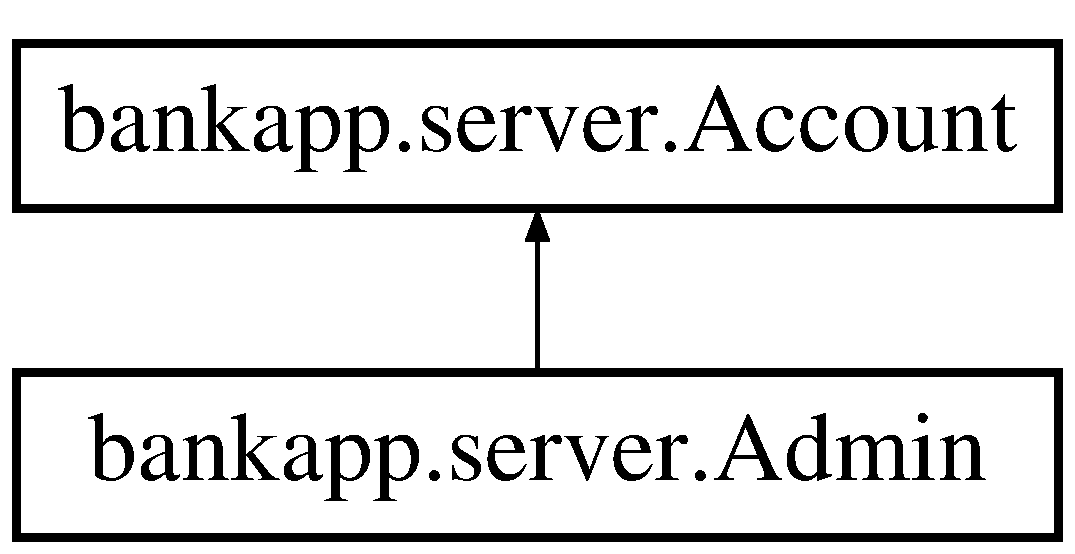
\includegraphics[height=2.000000cm]{classbankapp_1_1server_1_1_admin}
\end{center}
\end{figure}
\subsection*{Public Member Functions}
\begin{DoxyCompactItemize}
\item 
\hyperlink{classbankapp_1_1server_1_1_admin_a18a9fdce301d47d8f65febe728e2ae43}{Admin} (String username, String pass)
\end{DoxyCompactItemize}


\subsection{Detailed Description}


Definition at line 7 of file Admin.\+java.



\subsection{Constructor \& Destructor Documentation}
\mbox{\Hypertarget{classbankapp_1_1server_1_1_admin_a18a9fdce301d47d8f65febe728e2ae43}\label{classbankapp_1_1server_1_1_admin_a18a9fdce301d47d8f65febe728e2ae43}} 
\index{bankapp\+::server\+::\+Admin@{bankapp\+::server\+::\+Admin}!Admin@{Admin}}
\index{Admin@{Admin}!bankapp\+::server\+::\+Admin@{bankapp\+::server\+::\+Admin}}
\subsubsection{\texorpdfstring{Admin()}{Admin()}}
{\footnotesize\ttfamily bankapp.\+server.\+Admin.\+Admin (\begin{DoxyParamCaption}\item[{String}]{username,  }\item[{String}]{pass }\end{DoxyParamCaption})}



Definition at line 8 of file Admin.\+java.



The documentation for this class was generated from the following file\+:\begin{DoxyCompactItemize}
\item 
src/main/java/bankapp/server/\hyperlink{_admin_8java}{Admin.\+java}\end{DoxyCompactItemize}

\hypertarget{classbankapp_1_1server_1_1bank_account}{}\section{bankapp.\+server.\+bank\+Account Class Reference}
\label{classbankapp_1_1server_1_1bank_account}\index{bankapp.\+server.\+bank\+Account@{bankapp.\+server.\+bank\+Account}}
\subsection*{Public Member Functions}
\begin{DoxyCompactItemize}
\item 
\hyperlink{classbankapp_1_1server_1_1bank_account_ac69962d0e67c62d23bb1caa4ffd09d6b}{bank\+Account} ()
\item 
int \hyperlink{classbankapp_1_1server_1_1bank_account_a59c7532089ad72e06d43b3360d0f1ef4}{getnum\+Acc} ()
\item 
long \hyperlink{classbankapp_1_1server_1_1bank_account_ab66d3d80e858de46f26719628efa6ead}{getmoney} ()
\item 
void \hyperlink{classbankapp_1_1server_1_1bank_account_a1d9c03e89357753b211586186349dccf}{addmoney} (long money)
\item 
void \hyperlink{classbankapp_1_1server_1_1bank_account_ae68ea661e15b58e9843e72d6e71df834}{deducemoney} (long money)
\end{DoxyCompactItemize}


\subsection{Detailed Description}


Definition at line 6 of file bank\+Account.\+java.



\subsection{Constructor \& Destructor Documentation}
\mbox{\Hypertarget{classbankapp_1_1server_1_1bank_account_ac69962d0e67c62d23bb1caa4ffd09d6b}\label{classbankapp_1_1server_1_1bank_account_ac69962d0e67c62d23bb1caa4ffd09d6b}} 
\index{bankapp\+::server\+::bank\+Account@{bankapp\+::server\+::bank\+Account}!bank\+Account@{bank\+Account}}
\index{bank\+Account@{bank\+Account}!bankapp\+::server\+::bank\+Account@{bankapp\+::server\+::bank\+Account}}
\subsubsection{\texorpdfstring{bank\+Account()}{bankAccount()}}
{\footnotesize\ttfamily bankapp.\+server.\+bank\+Account.\+bank\+Account (\begin{DoxyParamCaption}{ }\end{DoxyParamCaption})}



Definition at line 11 of file bank\+Account.\+java.



\subsection{Member Function Documentation}
\mbox{\Hypertarget{classbankapp_1_1server_1_1bank_account_a1d9c03e89357753b211586186349dccf}\label{classbankapp_1_1server_1_1bank_account_a1d9c03e89357753b211586186349dccf}} 
\index{bankapp\+::server\+::bank\+Account@{bankapp\+::server\+::bank\+Account}!addmoney@{addmoney}}
\index{addmoney@{addmoney}!bankapp\+::server\+::bank\+Account@{bankapp\+::server\+::bank\+Account}}
\subsubsection{\texorpdfstring{addmoney()}{addmoney()}}
{\footnotesize\ttfamily void bankapp.\+server.\+bank\+Account.\+addmoney (\begin{DoxyParamCaption}\item[{long}]{money }\end{DoxyParamCaption})}



Definition at line 22 of file bank\+Account.\+java.

\mbox{\Hypertarget{classbankapp_1_1server_1_1bank_account_ae68ea661e15b58e9843e72d6e71df834}\label{classbankapp_1_1server_1_1bank_account_ae68ea661e15b58e9843e72d6e71df834}} 
\index{bankapp\+::server\+::bank\+Account@{bankapp\+::server\+::bank\+Account}!deducemoney@{deducemoney}}
\index{deducemoney@{deducemoney}!bankapp\+::server\+::bank\+Account@{bankapp\+::server\+::bank\+Account}}
\subsubsection{\texorpdfstring{deducemoney()}{deducemoney()}}
{\footnotesize\ttfamily void bankapp.\+server.\+bank\+Account.\+deducemoney (\begin{DoxyParamCaption}\item[{long}]{money }\end{DoxyParamCaption})}



Definition at line 25 of file bank\+Account.\+java.

\mbox{\Hypertarget{classbankapp_1_1server_1_1bank_account_ab66d3d80e858de46f26719628efa6ead}\label{classbankapp_1_1server_1_1bank_account_ab66d3d80e858de46f26719628efa6ead}} 
\index{bankapp\+::server\+::bank\+Account@{bankapp\+::server\+::bank\+Account}!getmoney@{getmoney}}
\index{getmoney@{getmoney}!bankapp\+::server\+::bank\+Account@{bankapp\+::server\+::bank\+Account}}
\subsubsection{\texorpdfstring{getmoney()}{getmoney()}}
{\footnotesize\ttfamily long bankapp.\+server.\+bank\+Account.\+getmoney (\begin{DoxyParamCaption}{ }\end{DoxyParamCaption})}



Definition at line 19 of file bank\+Account.\+java.

\mbox{\Hypertarget{classbankapp_1_1server_1_1bank_account_a59c7532089ad72e06d43b3360d0f1ef4}\label{classbankapp_1_1server_1_1bank_account_a59c7532089ad72e06d43b3360d0f1ef4}} 
\index{bankapp\+::server\+::bank\+Account@{bankapp\+::server\+::bank\+Account}!getnum\+Acc@{getnum\+Acc}}
\index{getnum\+Acc@{getnum\+Acc}!bankapp\+::server\+::bank\+Account@{bankapp\+::server\+::bank\+Account}}
\subsubsection{\texorpdfstring{getnum\+Acc()}{getnumAcc()}}
{\footnotesize\ttfamily int bankapp.\+server.\+bank\+Account.\+getnum\+Acc (\begin{DoxyParamCaption}{ }\end{DoxyParamCaption})}



Definition at line 16 of file bank\+Account.\+java.



The documentation for this class was generated from the following file\+:\begin{DoxyCompactItemize}
\item 
src/main/java/bankapp/server/\hyperlink{bank_account_8java}{bank\+Account.\+java}\end{DoxyCompactItemize}

\hypertarget{classbankapp_1_1server_1_1bank_account_test}{}\section{bankapp.\+server.\+bank\+Account\+Test Class Reference}
\label{classbankapp_1_1server_1_1bank_account_test}\index{bankapp.\+server.\+bank\+Account\+Test@{bankapp.\+server.\+bank\+Account\+Test}}
\subsection*{Public Member Functions}
\begin{DoxyCompactItemize}
\item 
void \hyperlink{classbankapp_1_1server_1_1bank_account_test_a3e13bd3f844ad027baa98092f5ed2b2a}{valid\+Account} ()
\end{DoxyCompactItemize}


\subsection{Detailed Description}


Definition at line 9 of file bank\+Account\+Test.\+java.



\subsection{Member Function Documentation}
\mbox{\Hypertarget{classbankapp_1_1server_1_1bank_account_test_a3e13bd3f844ad027baa98092f5ed2b2a}\label{classbankapp_1_1server_1_1bank_account_test_a3e13bd3f844ad027baa98092f5ed2b2a}} 
\index{bankapp\+::server\+::bank\+Account\+Test@{bankapp\+::server\+::bank\+Account\+Test}!valid\+Account@{valid\+Account}}
\index{valid\+Account@{valid\+Account}!bankapp\+::server\+::bank\+Account\+Test@{bankapp\+::server\+::bank\+Account\+Test}}
\subsubsection{\texorpdfstring{valid\+Account()}{validAccount()}}
{\footnotesize\ttfamily void bankapp.\+server.\+bank\+Account\+Test.\+valid\+Account (\begin{DoxyParamCaption}{ }\end{DoxyParamCaption})}



Definition at line 12 of file bank\+Account\+Test.\+java.



The documentation for this class was generated from the following file\+:\begin{DoxyCompactItemize}
\item 
src/test/java/bankapp/server/\hyperlink{bank_account_test_8java}{bank\+Account\+Test.\+java}\end{DoxyCompactItemize}

\hypertarget{classbankapp_1_1client_1_1bank_client}{}\section{bankapp.\+client.\+bank\+Client Class Reference}
\label{classbankapp_1_1client_1_1bank_client}\index{bankapp.\+client.\+bank\+Client@{bankapp.\+client.\+bank\+Client}}
\subsection*{Static Public Member Functions}
\begin{DoxyCompactItemize}
\item 
static void \hyperlink{classbankapp_1_1client_1_1bank_client_ad22392d35ad10f91cc417f169b69ff7b}{main} (String\mbox{[}$\,$\mbox{]} args)
\end{DoxyCompactItemize}


\subsection{Detailed Description}


Definition at line 5 of file Bank\+Client.\+java.



\subsection{Member Function Documentation}
\mbox{\Hypertarget{classbankapp_1_1client_1_1bank_client_ad22392d35ad10f91cc417f169b69ff7b}\label{classbankapp_1_1client_1_1bank_client_ad22392d35ad10f91cc417f169b69ff7b}} 
\index{bankapp\+::client\+::bank\+Client@{bankapp\+::client\+::bank\+Client}!main@{main}}
\index{main@{main}!bankapp\+::client\+::bank\+Client@{bankapp\+::client\+::bank\+Client}}
\subsubsection{\texorpdfstring{main()}{main()}}
{\footnotesize\ttfamily static void bankapp.\+client.\+bank\+Client.\+main (\begin{DoxyParamCaption}\item[{String \mbox{[}$\,$\mbox{]}}]{args }\end{DoxyParamCaption})\hspace{0.3cm}{\ttfamily [static]}}



Definition at line 8 of file Bank\+Client.\+java.



The documentation for this class was generated from the following file\+:\begin{DoxyCompactItemize}
\item 
src/main/java/bankapp/client/\hyperlink{_bank_client_8java}{Bank\+Client.\+java}\end{DoxyCompactItemize}

\hypertarget{classbankapp_1_1client_1_1bank_controller}{}\section{bankapp.\+client.\+bank\+Controller Class Reference}
\label{classbankapp_1_1client_1_1bank_controller}\index{bankapp.\+client.\+bank\+Controller@{bankapp.\+client.\+bank\+Controller}}
\subsection*{Public Member Functions}
\begin{DoxyCompactItemize}
\item 
\hyperlink{classbankapp_1_1client_1_1bank_controller_a632bf32141520837c5c06a2657a7c230}{bank\+Controller} (String ip, String port, String service\+Name)
\item 
boolean \hyperlink{classbankapp_1_1client_1_1bank_controller_aed80209fad3f3fee830107d259afb445}{login} (String user, String pass)
\end{DoxyCompactItemize}


\subsection{Detailed Description}


Definition at line 3 of file Bank\+Controller.\+java.



\subsection{Constructor \& Destructor Documentation}
\mbox{\Hypertarget{classbankapp_1_1client_1_1bank_controller_a632bf32141520837c5c06a2657a7c230}\label{classbankapp_1_1client_1_1bank_controller_a632bf32141520837c5c06a2657a7c230}} 
\index{bankapp\+::client\+::bank\+Controller@{bankapp\+::client\+::bank\+Controller}!bank\+Controller@{bank\+Controller}}
\index{bank\+Controller@{bank\+Controller}!bankapp\+::client\+::bank\+Controller@{bankapp\+::client\+::bank\+Controller}}
\subsubsection{\texorpdfstring{bank\+Controller()}{bankController()}}
{\footnotesize\ttfamily bankapp.\+client.\+bank\+Controller.\+bank\+Controller (\begin{DoxyParamCaption}\item[{String}]{ip,  }\item[{String}]{port,  }\item[{String}]{service\+Name }\end{DoxyParamCaption})}



Definition at line 7 of file Bank\+Controller.\+java.



\subsection{Member Function Documentation}
\mbox{\Hypertarget{classbankapp_1_1client_1_1bank_controller_aed80209fad3f3fee830107d259afb445}\label{classbankapp_1_1client_1_1bank_controller_aed80209fad3f3fee830107d259afb445}} 
\index{bankapp\+::client\+::bank\+Controller@{bankapp\+::client\+::bank\+Controller}!login@{login}}
\index{login@{login}!bankapp\+::client\+::bank\+Controller@{bankapp\+::client\+::bank\+Controller}}
\subsubsection{\texorpdfstring{login()}{login()}}
{\footnotesize\ttfamily boolean bankapp.\+client.\+bank\+Controller.\+login (\begin{DoxyParamCaption}\item[{String}]{user,  }\item[{String}]{pass }\end{DoxyParamCaption})}



Definition at line 14 of file Bank\+Controller.\+java.



The documentation for this class was generated from the following file\+:\begin{DoxyCompactItemize}
\item 
src/main/java/bankapp/client/\hyperlink{_bank_controller_8java}{Bank\+Controller.\+java}\end{DoxyCompactItemize}

\hypertarget{classbankapp_1_1server_1_1bank_d_a_o}{}\section{bankapp.\+server.\+bank\+D\+AO Class Reference}
\label{classbankapp_1_1server_1_1bank_d_a_o}\index{bankapp.\+server.\+bank\+D\+AO@{bankapp.\+server.\+bank\+D\+AO}}
Inheritance diagram for bankapp.\+server.\+bank\+D\+AO\+:\begin{figure}[H]
\begin{center}
\leavevmode
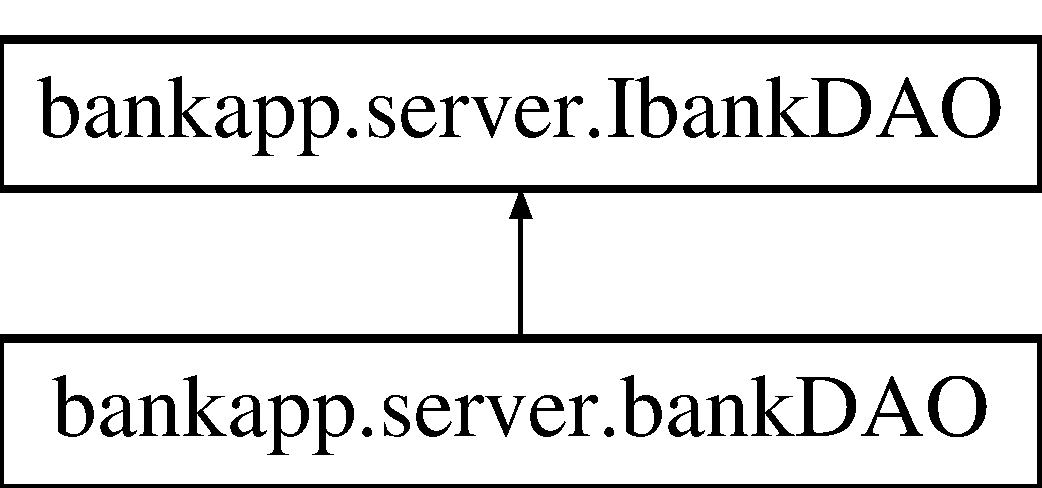
\includegraphics[height=2.000000cm]{classbankapp_1_1server_1_1bank_d_a_o}
\end{center}
\end{figure}
\subsection*{Public Member Functions}
\begin{DoxyCompactItemize}
\item 
\hyperlink{classbankapp_1_1server_1_1bank_d_a_o_a974c7da6eea192fb2f94a98a66e5068a}{bank\+D\+AO} ()
\item 
\hyperlink{classbankapp_1_1server_1_1_account}{Account} \hyperlink{classbankapp_1_1server_1_1bank_d_a_o_ad561ee843029636f739dbfad0bfb5414}{get\+Account} (String username)
\item 
void \hyperlink{classbankapp_1_1server_1_1bank_d_a_o_a0023f065d21c23dd9b952339fd832d7e}{store\+Account} (\hyperlink{classbankapp_1_1server_1_1_account}{Account} acc)
\item 
void \hyperlink{classbankapp_1_1server_1_1bank_d_a_o_a1909f3eb0622fb32291c0d1969bdf5df}{store\+Report} (\hyperlink{classbankapp_1_1server_1_1_report}{Report} rep)
\item 
void \hyperlink{classbankapp_1_1server_1_1bank_d_a_o_a3c6e87d45ba675ea26be1d7227de0183}{delete\+Account} (String username)
\end{DoxyCompactItemize}


\subsection{Detailed Description}


Definition at line 13 of file Bank\+D\+A\+O.\+java.



\subsection{Constructor \& Destructor Documentation}
\mbox{\Hypertarget{classbankapp_1_1server_1_1bank_d_a_o_a974c7da6eea192fb2f94a98a66e5068a}\label{classbankapp_1_1server_1_1bank_d_a_o_a974c7da6eea192fb2f94a98a66e5068a}} 
\index{bankapp\+::server\+::bank\+D\+AO@{bankapp\+::server\+::bank\+D\+AO}!bank\+D\+AO@{bank\+D\+AO}}
\index{bank\+D\+AO@{bank\+D\+AO}!bankapp\+::server\+::bank\+D\+AO@{bankapp\+::server\+::bank\+D\+AO}}
\subsubsection{\texorpdfstring{bank\+D\+A\+O()}{bankDAO()}}
{\footnotesize\ttfamily bankapp.\+server.\+bank\+D\+A\+O.\+bank\+D\+AO (\begin{DoxyParamCaption}{ }\end{DoxyParamCaption})}



Definition at line 15 of file Bank\+D\+A\+O.\+java.



\subsection{Member Function Documentation}
\mbox{\Hypertarget{classbankapp_1_1server_1_1bank_d_a_o_a3c6e87d45ba675ea26be1d7227de0183}\label{classbankapp_1_1server_1_1bank_d_a_o_a3c6e87d45ba675ea26be1d7227de0183}} 
\index{bankapp\+::server\+::bank\+D\+AO@{bankapp\+::server\+::bank\+D\+AO}!delete\+Account@{delete\+Account}}
\index{delete\+Account@{delete\+Account}!bankapp\+::server\+::bank\+D\+AO@{bankapp\+::server\+::bank\+D\+AO}}
\subsubsection{\texorpdfstring{delete\+Account()}{deleteAccount()}}
{\footnotesize\ttfamily void bankapp.\+server.\+bank\+D\+A\+O.\+delete\+Account (\begin{DoxyParamCaption}\item[{String}]{username }\end{DoxyParamCaption})}



Implements \hyperlink{interfacebankapp_1_1server_1_1_ibank_d_a_o_a618b28f4d950f4d2705745c13d7be470}{bankapp.\+server.\+Ibank\+D\+AO}.



Definition at line 87 of file Bank\+D\+A\+O.\+java.

\mbox{\Hypertarget{classbankapp_1_1server_1_1bank_d_a_o_ad561ee843029636f739dbfad0bfb5414}\label{classbankapp_1_1server_1_1bank_d_a_o_ad561ee843029636f739dbfad0bfb5414}} 
\index{bankapp\+::server\+::bank\+D\+AO@{bankapp\+::server\+::bank\+D\+AO}!get\+Account@{get\+Account}}
\index{get\+Account@{get\+Account}!bankapp\+::server\+::bank\+D\+AO@{bankapp\+::server\+::bank\+D\+AO}}
\subsubsection{\texorpdfstring{get\+Account()}{getAccount()}}
{\footnotesize\ttfamily \hyperlink{classbankapp_1_1server_1_1_account}{Account} bankapp.\+server.\+bank\+D\+A\+O.\+get\+Account (\begin{DoxyParamCaption}\item[{String}]{username }\end{DoxyParamCaption})}



Implements \hyperlink{interfacebankapp_1_1server_1_1_ibank_d_a_o_af0e84b74c8826ce5fb80a156bc19e488}{bankapp.\+server.\+Ibank\+D\+AO}.



Definition at line 21 of file Bank\+D\+A\+O.\+java.

\mbox{\Hypertarget{classbankapp_1_1server_1_1bank_d_a_o_a0023f065d21c23dd9b952339fd832d7e}\label{classbankapp_1_1server_1_1bank_d_a_o_a0023f065d21c23dd9b952339fd832d7e}} 
\index{bankapp\+::server\+::bank\+D\+AO@{bankapp\+::server\+::bank\+D\+AO}!store\+Account@{store\+Account}}
\index{store\+Account@{store\+Account}!bankapp\+::server\+::bank\+D\+AO@{bankapp\+::server\+::bank\+D\+AO}}
\subsubsection{\texorpdfstring{store\+Account()}{storeAccount()}}
{\footnotesize\ttfamily void bankapp.\+server.\+bank\+D\+A\+O.\+store\+Account (\begin{DoxyParamCaption}\item[{\hyperlink{classbankapp_1_1server_1_1_account}{Account}}]{acc }\end{DoxyParamCaption})}



Implements \hyperlink{interfacebankapp_1_1server_1_1_ibank_d_a_o_a6631fb11c78a48b05a743e4f7f2757ef}{bankapp.\+server.\+Ibank\+D\+AO}.



Definition at line 46 of file Bank\+D\+A\+O.\+java.

\mbox{\Hypertarget{classbankapp_1_1server_1_1bank_d_a_o_a1909f3eb0622fb32291c0d1969bdf5df}\label{classbankapp_1_1server_1_1bank_d_a_o_a1909f3eb0622fb32291c0d1969bdf5df}} 
\index{bankapp\+::server\+::bank\+D\+AO@{bankapp\+::server\+::bank\+D\+AO}!store\+Report@{store\+Report}}
\index{store\+Report@{store\+Report}!bankapp\+::server\+::bank\+D\+AO@{bankapp\+::server\+::bank\+D\+AO}}
\subsubsection{\texorpdfstring{store\+Report()}{storeReport()}}
{\footnotesize\ttfamily void bankapp.\+server.\+bank\+D\+A\+O.\+store\+Report (\begin{DoxyParamCaption}\item[{\hyperlink{classbankapp_1_1server_1_1_report}{Report}}]{rep }\end{DoxyParamCaption})}



Implements \hyperlink{interfacebankapp_1_1server_1_1_ibank_d_a_o_a8990d1f4e0ffb741d459cebe172e47e0}{bankapp.\+server.\+Ibank\+D\+AO}.



Definition at line 66 of file Bank\+D\+A\+O.\+java.



The documentation for this class was generated from the following file\+:\begin{DoxyCompactItemize}
\item 
src/main/java/bankapp/server/\hyperlink{_bank_d_a_o_8java}{Bank\+D\+A\+O.\+java}\end{DoxyCompactItemize}

\hypertarget{classbankapp_1_1server_1_1bank_server}{}\section{bankapp.\+server.\+bank\+Server Class Reference}
\label{classbankapp_1_1server_1_1bank_server}\index{bankapp.\+server.\+bank\+Server@{bankapp.\+server.\+bank\+Server}}
\subsection*{Static Public Member Functions}
\begin{DoxyCompactItemize}
\item 
static void \hyperlink{classbankapp_1_1server_1_1bank_server_aca6d24bb05576a3668a4421453785f90}{main} (String args\mbox{[}$\,$\mbox{]})
\end{DoxyCompactItemize}


\subsection{Detailed Description}


Definition at line 6 of file Bank\+Server.\+java.



\subsection{Member Function Documentation}
\mbox{\Hypertarget{classbankapp_1_1server_1_1bank_server_aca6d24bb05576a3668a4421453785f90}\label{classbankapp_1_1server_1_1bank_server_aca6d24bb05576a3668a4421453785f90}} 
\index{bankapp\+::server\+::bank\+Server@{bankapp\+::server\+::bank\+Server}!main@{main}}
\index{main@{main}!bankapp\+::server\+::bank\+Server@{bankapp\+::server\+::bank\+Server}}
\subsubsection{\texorpdfstring{main()}{main()}}
{\footnotesize\ttfamily static void bankapp.\+server.\+bank\+Server.\+main (\begin{DoxyParamCaption}\item[{String}]{args\mbox{[}$\,$\mbox{]} }\end{DoxyParamCaption})\hspace{0.3cm}{\ttfamily [static]}}



Definition at line 7 of file Bank\+Server.\+java.



The documentation for this class was generated from the following file\+:\begin{DoxyCompactItemize}
\item 
src/main/java/bankapp/server/\hyperlink{_bank_server_8java}{Bank\+Server.\+java}\end{DoxyCompactItemize}

\hypertarget{classbankapp_1_1server_1_1_b_d_test}{}\section{bankapp.\+server.\+B\+D\+Test Class Reference}
\label{classbankapp_1_1server_1_1_b_d_test}\index{bankapp.\+server.\+B\+D\+Test@{bankapp.\+server.\+B\+D\+Test}}
\subsection*{Public Member Functions}
\begin{DoxyCompactItemize}
\item 
void \hyperlink{classbankapp_1_1server_1_1_b_d_test_a35da4c83723ff5395b80cd0b2a65bde3}{setup} ()
\item 
void \hyperlink{classbankapp_1_1server_1_1_b_d_test_a1f849eef20082450ec61a7a54fd50865}{valid\+BD} ()
\end{DoxyCompactItemize}


\subsection{Detailed Description}


Definition at line 8 of file B\+D\+Test.\+java.



\subsection{Member Function Documentation}
\mbox{\Hypertarget{classbankapp_1_1server_1_1_b_d_test_a35da4c83723ff5395b80cd0b2a65bde3}\label{classbankapp_1_1server_1_1_b_d_test_a35da4c83723ff5395b80cd0b2a65bde3}} 
\index{bankapp\+::server\+::\+B\+D\+Test@{bankapp\+::server\+::\+B\+D\+Test}!setup@{setup}}
\index{setup@{setup}!bankapp\+::server\+::\+B\+D\+Test@{bankapp\+::server\+::\+B\+D\+Test}}
\subsubsection{\texorpdfstring{setup()}{setup()}}
{\footnotesize\ttfamily void bankapp.\+server.\+B\+D\+Test.\+setup (\begin{DoxyParamCaption}{ }\end{DoxyParamCaption})}



Definition at line 11 of file B\+D\+Test.\+java.

\mbox{\Hypertarget{classbankapp_1_1server_1_1_b_d_test_a1f849eef20082450ec61a7a54fd50865}\label{classbankapp_1_1server_1_1_b_d_test_a1f849eef20082450ec61a7a54fd50865}} 
\index{bankapp\+::server\+::\+B\+D\+Test@{bankapp\+::server\+::\+B\+D\+Test}!valid\+BD@{valid\+BD}}
\index{valid\+BD@{valid\+BD}!bankapp\+::server\+::\+B\+D\+Test@{bankapp\+::server\+::\+B\+D\+Test}}
\subsubsection{\texorpdfstring{valid\+B\+D()}{validBD()}}
{\footnotesize\ttfamily void bankapp.\+server.\+B\+D\+Test.\+valid\+BD (\begin{DoxyParamCaption}{ }\end{DoxyParamCaption})}



Definition at line 16 of file B\+D\+Test.\+java.



The documentation for this class was generated from the following file\+:\begin{DoxyCompactItemize}
\item 
src/test/java/bankapp/server/\hyperlink{_b_d_test_8java}{B\+D\+Test.\+java}\end{DoxyCompactItemize}

\hypertarget{classbankapp_1_1server_1_1_b_manager}{}\section{bankapp.\+server.\+B\+Manager Class Reference}
\label{classbankapp_1_1server_1_1_b_manager}\index{bankapp.\+server.\+B\+Manager@{bankapp.\+server.\+B\+Manager}}
Inheritance diagram for bankapp.\+server.\+B\+Manager\+:\begin{figure}[H]
\begin{center}
\leavevmode
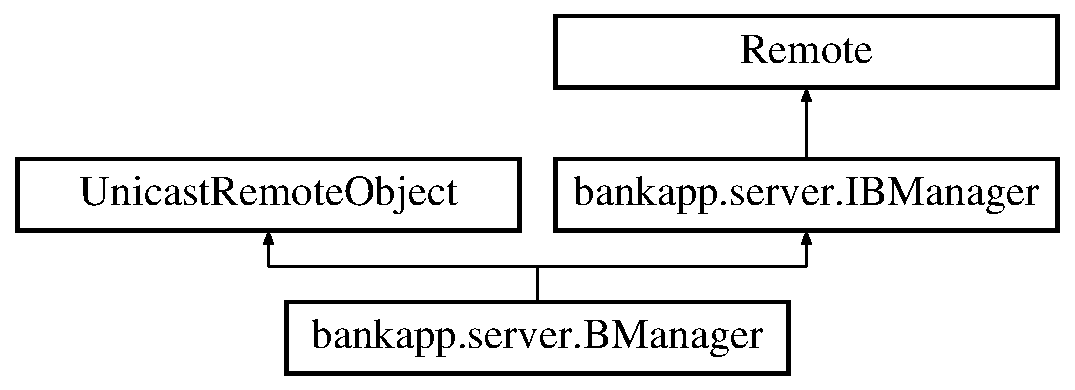
\includegraphics[height=3.000000cm]{classbankapp_1_1server_1_1_b_manager}
\end{center}
\end{figure}
\subsection*{Public Member Functions}
\begin{DoxyCompactItemize}
\item 
\hyperlink{classbankapp_1_1server_1_1_b_manager_aa7f45d3eddae4e91afaf2b19275b0c7e}{B\+Manager} (String server\+Address, String port0, String serv\+Name)  throws Remote\+Exception 
\item 
char \hyperlink{classbankapp_1_1server_1_1_b_manager_a3840891c318887cef8ed2f7c193cfba9}{login} (String username, String pass)  throws Remote\+Exception 
\item 
void \hyperlink{classbankapp_1_1server_1_1_b_manager_a5ce24fa69bd4bd08ef793072495b84b4}{transaction} (String user1, String user2, long money, String acc\+Num1, String acc\+Num2)  throws Remote\+Exception 
\item 
int \hyperlink{classbankapp_1_1server_1_1_b_manager_abf7716d220d573ad491f4ee15312aaff}{create\+Bank\+Account} (String user)  throws Remote\+Exception 
\item 
void \hyperlink{classbankapp_1_1server_1_1_b_manager_a0c81d9fb02961e95efa371249f284b47}{add\+Funds} (String user, String acc\+Num, long money)  throws Remote\+Exception 
\item 
void \hyperlink{classbankapp_1_1server_1_1_b_manager_a56404dc8a349618d517f73ad4f8e0026}{delete\+Bank\+Account} (String user, String acc\+Num1, String acc\+Num2)  throws Remote\+Exception 
\item 
void \hyperlink{classbankapp_1_1server_1_1_b_manager_ad8c5c164841d3ad7e25070c6b065bb4d}{delete\+Account} (String user)  throws Remote\+Exception 
\item 
void \hyperlink{classbankapp_1_1server_1_1_b_manager_ad98f4af0b4ae0842a58570e6c08a371c}{create\+User} (String username, String pass, String email)  throws Remote\+Exception 
\end{DoxyCompactItemize}


\subsection{Detailed Description}


Definition at line 8 of file B\+Manager.\+java.



\subsection{Constructor \& Destructor Documentation}
\mbox{\Hypertarget{classbankapp_1_1server_1_1_b_manager_aa7f45d3eddae4e91afaf2b19275b0c7e}\label{classbankapp_1_1server_1_1_b_manager_aa7f45d3eddae4e91afaf2b19275b0c7e}} 
\index{bankapp\+::server\+::\+B\+Manager@{bankapp\+::server\+::\+B\+Manager}!B\+Manager@{B\+Manager}}
\index{B\+Manager@{B\+Manager}!bankapp\+::server\+::\+B\+Manager@{bankapp\+::server\+::\+B\+Manager}}
\subsubsection{\texorpdfstring{B\+Manager()}{BManager()}}
{\footnotesize\ttfamily bankapp.\+server.\+B\+Manager.\+B\+Manager (\begin{DoxyParamCaption}\item[{String}]{server\+Address,  }\item[{String}]{port0,  }\item[{String}]{serv\+Name }\end{DoxyParamCaption}) throws Remote\+Exception}



Definition at line 22 of file B\+Manager.\+java.



\subsection{Member Function Documentation}
\mbox{\Hypertarget{classbankapp_1_1server_1_1_b_manager_a0c81d9fb02961e95efa371249f284b47}\label{classbankapp_1_1server_1_1_b_manager_a0c81d9fb02961e95efa371249f284b47}} 
\index{bankapp\+::server\+::\+B\+Manager@{bankapp\+::server\+::\+B\+Manager}!add\+Funds@{add\+Funds}}
\index{add\+Funds@{add\+Funds}!bankapp\+::server\+::\+B\+Manager@{bankapp\+::server\+::\+B\+Manager}}
\subsubsection{\texorpdfstring{add\+Funds()}{addFunds()}}
{\footnotesize\ttfamily void bankapp.\+server.\+B\+Manager.\+add\+Funds (\begin{DoxyParamCaption}\item[{String}]{user,  }\item[{String}]{acc\+Num,  }\item[{long}]{money }\end{DoxyParamCaption}) throws Remote\+Exception}



Implements \hyperlink{interfacebankapp_1_1server_1_1_i_b_manager_a31f275bed15b74bb2bc6ef43ede7f7f8}{bankapp.\+server.\+I\+B\+Manager}.



Definition at line 79 of file B\+Manager.\+java.

\mbox{\Hypertarget{classbankapp_1_1server_1_1_b_manager_abf7716d220d573ad491f4ee15312aaff}\label{classbankapp_1_1server_1_1_b_manager_abf7716d220d573ad491f4ee15312aaff}} 
\index{bankapp\+::server\+::\+B\+Manager@{bankapp\+::server\+::\+B\+Manager}!create\+Bank\+Account@{create\+Bank\+Account}}
\index{create\+Bank\+Account@{create\+Bank\+Account}!bankapp\+::server\+::\+B\+Manager@{bankapp\+::server\+::\+B\+Manager}}
\subsubsection{\texorpdfstring{create\+Bank\+Account()}{createBankAccount()}}
{\footnotesize\ttfamily int bankapp.\+server.\+B\+Manager.\+create\+Bank\+Account (\begin{DoxyParamCaption}\item[{String}]{user }\end{DoxyParamCaption}) throws Remote\+Exception}



Implements \hyperlink{interfacebankapp_1_1server_1_1_i_b_manager_aeb423a1ba2348fdaa7d1466a907e82e1}{bankapp.\+server.\+I\+B\+Manager}.



Definition at line 70 of file B\+Manager.\+java.

\mbox{\Hypertarget{classbankapp_1_1server_1_1_b_manager_ad98f4af0b4ae0842a58570e6c08a371c}\label{classbankapp_1_1server_1_1_b_manager_ad98f4af0b4ae0842a58570e6c08a371c}} 
\index{bankapp\+::server\+::\+B\+Manager@{bankapp\+::server\+::\+B\+Manager}!create\+User@{create\+User}}
\index{create\+User@{create\+User}!bankapp\+::server\+::\+B\+Manager@{bankapp\+::server\+::\+B\+Manager}}
\subsubsection{\texorpdfstring{create\+User()}{createUser()}}
{\footnotesize\ttfamily void bankapp.\+server.\+B\+Manager.\+create\+User (\begin{DoxyParamCaption}\item[{String}]{username,  }\item[{String}]{pass,  }\item[{String}]{email }\end{DoxyParamCaption}) throws Remote\+Exception}



Implements \hyperlink{interfacebankapp_1_1server_1_1_i_b_manager_a09b3ca29b50f7c662e360a47cea220ae}{bankapp.\+server.\+I\+B\+Manager}.



Definition at line 103 of file B\+Manager.\+java.

\mbox{\Hypertarget{classbankapp_1_1server_1_1_b_manager_ad8c5c164841d3ad7e25070c6b065bb4d}\label{classbankapp_1_1server_1_1_b_manager_ad8c5c164841d3ad7e25070c6b065bb4d}} 
\index{bankapp\+::server\+::\+B\+Manager@{bankapp\+::server\+::\+B\+Manager}!delete\+Account@{delete\+Account}}
\index{delete\+Account@{delete\+Account}!bankapp\+::server\+::\+B\+Manager@{bankapp\+::server\+::\+B\+Manager}}
\subsubsection{\texorpdfstring{delete\+Account()}{deleteAccount()}}
{\footnotesize\ttfamily void bankapp.\+server.\+B\+Manager.\+delete\+Account (\begin{DoxyParamCaption}\item[{String}]{user }\end{DoxyParamCaption}) throws Remote\+Exception}



Implements \hyperlink{interfacebankapp_1_1server_1_1_i_b_manager_aa1f1aee23930d78375c12496e9f47cdf}{bankapp.\+server.\+I\+B\+Manager}.



Definition at line 97 of file B\+Manager.\+java.

\mbox{\Hypertarget{classbankapp_1_1server_1_1_b_manager_a56404dc8a349618d517f73ad4f8e0026}\label{classbankapp_1_1server_1_1_b_manager_a56404dc8a349618d517f73ad4f8e0026}} 
\index{bankapp\+::server\+::\+B\+Manager@{bankapp\+::server\+::\+B\+Manager}!delete\+Bank\+Account@{delete\+Bank\+Account}}
\index{delete\+Bank\+Account@{delete\+Bank\+Account}!bankapp\+::server\+::\+B\+Manager@{bankapp\+::server\+::\+B\+Manager}}
\subsubsection{\texorpdfstring{delete\+Bank\+Account()}{deleteBankAccount()}}
{\footnotesize\ttfamily void bankapp.\+server.\+B\+Manager.\+delete\+Bank\+Account (\begin{DoxyParamCaption}\item[{String}]{user,  }\item[{String}]{acc\+Num1,  }\item[{String}]{acc\+Num2 }\end{DoxyParamCaption}) throws Remote\+Exception}



Implements \hyperlink{interfacebankapp_1_1server_1_1_i_b_manager_a7b1a8e3d663126a894a7c074f35e49d3}{bankapp.\+server.\+I\+B\+Manager}.



Definition at line 88 of file B\+Manager.\+java.

\mbox{\Hypertarget{classbankapp_1_1server_1_1_b_manager_a3840891c318887cef8ed2f7c193cfba9}\label{classbankapp_1_1server_1_1_b_manager_a3840891c318887cef8ed2f7c193cfba9}} 
\index{bankapp\+::server\+::\+B\+Manager@{bankapp\+::server\+::\+B\+Manager}!login@{login}}
\index{login@{login}!bankapp\+::server\+::\+B\+Manager@{bankapp\+::server\+::\+B\+Manager}}
\subsubsection{\texorpdfstring{login()}{login()}}
{\footnotesize\ttfamily char bankapp.\+server.\+B\+Manager.\+login (\begin{DoxyParamCaption}\item[{String}]{username,  }\item[{String}]{pass }\end{DoxyParamCaption}) throws Remote\+Exception}



Implements \hyperlink{interfacebankapp_1_1server_1_1_i_b_manager_a96bce16e21db1585eb42a5ef55b43050}{bankapp.\+server.\+I\+B\+Manager}.



Definition at line 30 of file B\+Manager.\+java.

\mbox{\Hypertarget{classbankapp_1_1server_1_1_b_manager_a5ce24fa69bd4bd08ef793072495b84b4}\label{classbankapp_1_1server_1_1_b_manager_a5ce24fa69bd4bd08ef793072495b84b4}} 
\index{bankapp\+::server\+::\+B\+Manager@{bankapp\+::server\+::\+B\+Manager}!transaction@{transaction}}
\index{transaction@{transaction}!bankapp\+::server\+::\+B\+Manager@{bankapp\+::server\+::\+B\+Manager}}
\subsubsection{\texorpdfstring{transaction()}{transaction()}}
{\footnotesize\ttfamily void bankapp.\+server.\+B\+Manager.\+transaction (\begin{DoxyParamCaption}\item[{String}]{user1,  }\item[{String}]{user2,  }\item[{long}]{money,  }\item[{String}]{acc\+Num1,  }\item[{String}]{acc\+Num2 }\end{DoxyParamCaption}) throws Remote\+Exception}



Implements \hyperlink{interfacebankapp_1_1server_1_1_i_b_manager_a6ed6af471750f7c721d45ead983bef5d}{bankapp.\+server.\+I\+B\+Manager}.



Definition at line 53 of file B\+Manager.\+java.



The documentation for this class was generated from the following file\+:\begin{DoxyCompactItemize}
\item 
src/main/java/bankapp/server/\hyperlink{_b_manager_8java}{B\+Manager.\+java}\end{DoxyCompactItemize}

\hypertarget{interfacebankapp_1_1server_1_1_ibank_d_a_o}{}\section{bankapp.\+server.\+Ibank\+D\+AO Interface Reference}
\label{interfacebankapp_1_1server_1_1_ibank_d_a_o}\index{bankapp.\+server.\+Ibank\+D\+AO@{bankapp.\+server.\+Ibank\+D\+AO}}
Inheritance diagram for bankapp.\+server.\+Ibank\+D\+AO\+:\begin{figure}[H]
\begin{center}
\leavevmode
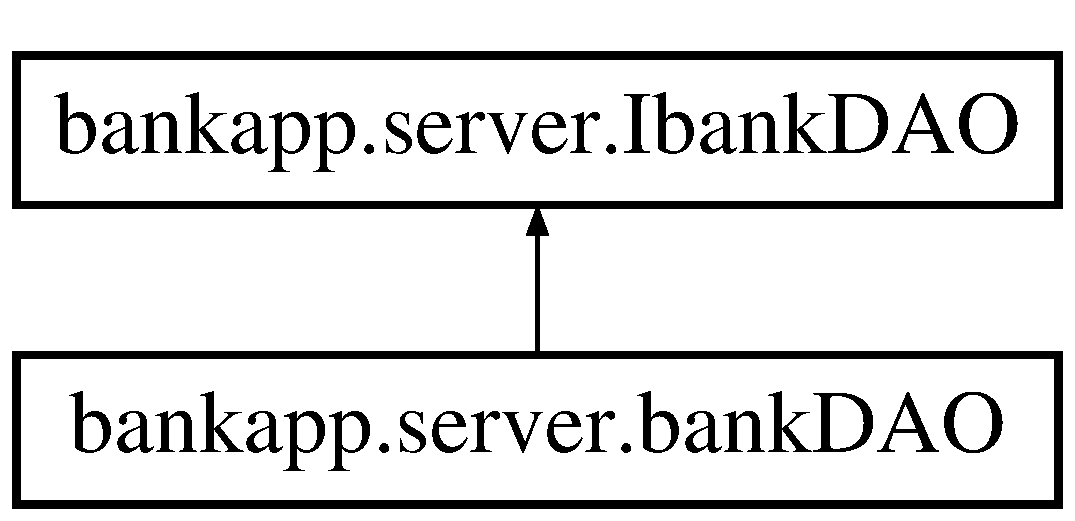
\includegraphics[height=2.000000cm]{interfacebankapp_1_1server_1_1_ibank_d_a_o}
\end{center}
\end{figure}
\subsection*{Public Member Functions}
\begin{DoxyCompactItemize}
\item 
\hyperlink{classbankapp_1_1server_1_1_account}{Account} \hyperlink{interfacebankapp_1_1server_1_1_ibank_d_a_o_af0e84b74c8826ce5fb80a156bc19e488}{get\+Account} (String username)
\item 
void \hyperlink{interfacebankapp_1_1server_1_1_ibank_d_a_o_a6631fb11c78a48b05a743e4f7f2757ef}{store\+Account} (\hyperlink{classbankapp_1_1server_1_1_account}{Account} acc)
\item 
void \hyperlink{interfacebankapp_1_1server_1_1_ibank_d_a_o_a8990d1f4e0ffb741d459cebe172e47e0}{store\+Report} (\hyperlink{classbankapp_1_1server_1_1_report}{Report} rep)
\item 
void \hyperlink{interfacebankapp_1_1server_1_1_ibank_d_a_o_a618b28f4d950f4d2705745c13d7be470}{delete\+Account} (String username)
\end{DoxyCompactItemize}


\subsection{Detailed Description}


Definition at line 4 of file I\+Bank\+D\+A\+O.\+java.



\subsection{Member Function Documentation}
\mbox{\Hypertarget{interfacebankapp_1_1server_1_1_ibank_d_a_o_a618b28f4d950f4d2705745c13d7be470}\label{interfacebankapp_1_1server_1_1_ibank_d_a_o_a618b28f4d950f4d2705745c13d7be470}} 
\index{bankapp\+::server\+::\+Ibank\+D\+AO@{bankapp\+::server\+::\+Ibank\+D\+AO}!delete\+Account@{delete\+Account}}
\index{delete\+Account@{delete\+Account}!bankapp\+::server\+::\+Ibank\+D\+AO@{bankapp\+::server\+::\+Ibank\+D\+AO}}
\subsubsection{\texorpdfstring{delete\+Account()}{deleteAccount()}}
{\footnotesize\ttfamily void bankapp.\+server.\+Ibank\+D\+A\+O.\+delete\+Account (\begin{DoxyParamCaption}\item[{String}]{username }\end{DoxyParamCaption})}



Implemented in \hyperlink{classbankapp_1_1server_1_1bank_d_a_o_a3c6e87d45ba675ea26be1d7227de0183}{bankapp.\+server.\+bank\+D\+AO}.

\mbox{\Hypertarget{interfacebankapp_1_1server_1_1_ibank_d_a_o_af0e84b74c8826ce5fb80a156bc19e488}\label{interfacebankapp_1_1server_1_1_ibank_d_a_o_af0e84b74c8826ce5fb80a156bc19e488}} 
\index{bankapp\+::server\+::\+Ibank\+D\+AO@{bankapp\+::server\+::\+Ibank\+D\+AO}!get\+Account@{get\+Account}}
\index{get\+Account@{get\+Account}!bankapp\+::server\+::\+Ibank\+D\+AO@{bankapp\+::server\+::\+Ibank\+D\+AO}}
\subsubsection{\texorpdfstring{get\+Account()}{getAccount()}}
{\footnotesize\ttfamily \hyperlink{classbankapp_1_1server_1_1_account}{Account} bankapp.\+server.\+Ibank\+D\+A\+O.\+get\+Account (\begin{DoxyParamCaption}\item[{String}]{username }\end{DoxyParamCaption})}



Implemented in \hyperlink{classbankapp_1_1server_1_1bank_d_a_o_ad561ee843029636f739dbfad0bfb5414}{bankapp.\+server.\+bank\+D\+AO}.

\mbox{\Hypertarget{interfacebankapp_1_1server_1_1_ibank_d_a_o_a6631fb11c78a48b05a743e4f7f2757ef}\label{interfacebankapp_1_1server_1_1_ibank_d_a_o_a6631fb11c78a48b05a743e4f7f2757ef}} 
\index{bankapp\+::server\+::\+Ibank\+D\+AO@{bankapp\+::server\+::\+Ibank\+D\+AO}!store\+Account@{store\+Account}}
\index{store\+Account@{store\+Account}!bankapp\+::server\+::\+Ibank\+D\+AO@{bankapp\+::server\+::\+Ibank\+D\+AO}}
\subsubsection{\texorpdfstring{store\+Account()}{storeAccount()}}
{\footnotesize\ttfamily void bankapp.\+server.\+Ibank\+D\+A\+O.\+store\+Account (\begin{DoxyParamCaption}\item[{\hyperlink{classbankapp_1_1server_1_1_account}{Account}}]{acc }\end{DoxyParamCaption})}



Implemented in \hyperlink{classbankapp_1_1server_1_1bank_d_a_o_a0023f065d21c23dd9b952339fd832d7e}{bankapp.\+server.\+bank\+D\+AO}.

\mbox{\Hypertarget{interfacebankapp_1_1server_1_1_ibank_d_a_o_a8990d1f4e0ffb741d459cebe172e47e0}\label{interfacebankapp_1_1server_1_1_ibank_d_a_o_a8990d1f4e0ffb741d459cebe172e47e0}} 
\index{bankapp\+::server\+::\+Ibank\+D\+AO@{bankapp\+::server\+::\+Ibank\+D\+AO}!store\+Report@{store\+Report}}
\index{store\+Report@{store\+Report}!bankapp\+::server\+::\+Ibank\+D\+AO@{bankapp\+::server\+::\+Ibank\+D\+AO}}
\subsubsection{\texorpdfstring{store\+Report()}{storeReport()}}
{\footnotesize\ttfamily void bankapp.\+server.\+Ibank\+D\+A\+O.\+store\+Report (\begin{DoxyParamCaption}\item[{\hyperlink{classbankapp_1_1server_1_1_report}{Report}}]{rep }\end{DoxyParamCaption})}



Implemented in \hyperlink{classbankapp_1_1server_1_1bank_d_a_o_a1909f3eb0622fb32291c0d1969bdf5df}{bankapp.\+server.\+bank\+D\+AO}.



The documentation for this interface was generated from the following file\+:\begin{DoxyCompactItemize}
\item 
src/main/java/bankapp/server/\hyperlink{_i_bank_d_a_o_8java}{I\+Bank\+D\+A\+O.\+java}\end{DoxyCompactItemize}

\hypertarget{interfacebankapp_1_1server_1_1_i_b_manager}{}\section{bankapp.\+server.\+I\+B\+Manager Interface Reference}
\label{interfacebankapp_1_1server_1_1_i_b_manager}\index{bankapp.\+server.\+I\+B\+Manager@{bankapp.\+server.\+I\+B\+Manager}}
Inheritance diagram for bankapp.\+server.\+I\+B\+Manager\+:\begin{figure}[H]
\begin{center}
\leavevmode
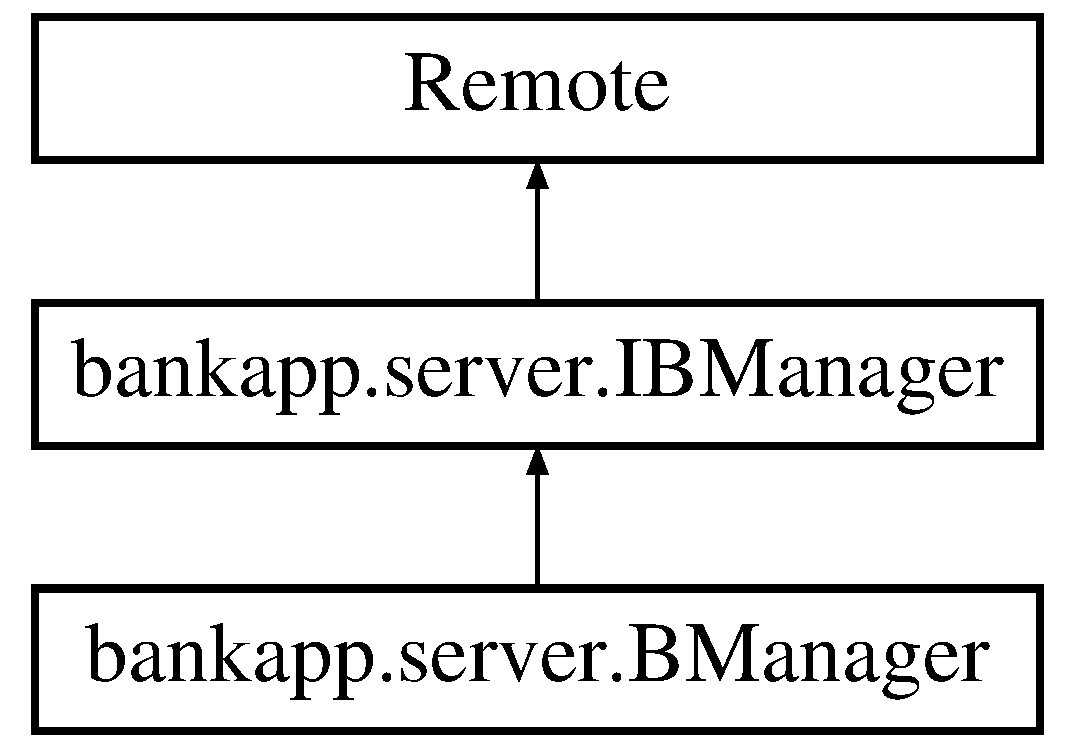
\includegraphics[height=3.000000cm]{interfacebankapp_1_1server_1_1_i_b_manager}
\end{center}
\end{figure}
\subsection*{Public Member Functions}
\begin{DoxyCompactItemize}
\item 
char \hyperlink{interfacebankapp_1_1server_1_1_i_b_manager_a96bce16e21db1585eb42a5ef55b43050}{login} (String user, String pass)  throws Remote\+Exception
\item 
void \hyperlink{interfacebankapp_1_1server_1_1_i_b_manager_a6ed6af471750f7c721d45ead983bef5d}{transaction} (String user1, String user2, long money, String acc\+Num1, String acc\+Num2)  throws Remote\+Exception
\item 
int \hyperlink{interfacebankapp_1_1server_1_1_i_b_manager_aeb423a1ba2348fdaa7d1466a907e82e1}{create\+Bank\+Account} (String user)  throws Remote\+Exception
\item 
void \hyperlink{interfacebankapp_1_1server_1_1_i_b_manager_a31f275bed15b74bb2bc6ef43ede7f7f8}{add\+Funds} (String user, String acc\+Num, long money)  throws Remote\+Exception
\item 
void \hyperlink{interfacebankapp_1_1server_1_1_i_b_manager_a7b1a8e3d663126a894a7c074f35e49d3}{delete\+Bank\+Account} (String user, String acc\+Num1, String acc\+Num2)  throws Remote\+Exception
\item 
void \hyperlink{interfacebankapp_1_1server_1_1_i_b_manager_aa1f1aee23930d78375c12496e9f47cdf}{delete\+Account} (String user)  throws Remote\+Exception
\item 
void \hyperlink{interfacebankapp_1_1server_1_1_i_b_manager_a09b3ca29b50f7c662e360a47cea220ae}{create\+User} (String username, String pass, String email)  throws Remote\+Exception
\end{DoxyCompactItemize}


\subsection{Detailed Description}


Definition at line 6 of file I\+B\+Manager.\+java.



\subsection{Member Function Documentation}
\mbox{\Hypertarget{interfacebankapp_1_1server_1_1_i_b_manager_a31f275bed15b74bb2bc6ef43ede7f7f8}\label{interfacebankapp_1_1server_1_1_i_b_manager_a31f275bed15b74bb2bc6ef43ede7f7f8}} 
\index{bankapp\+::server\+::\+I\+B\+Manager@{bankapp\+::server\+::\+I\+B\+Manager}!add\+Funds@{add\+Funds}}
\index{add\+Funds@{add\+Funds}!bankapp\+::server\+::\+I\+B\+Manager@{bankapp\+::server\+::\+I\+B\+Manager}}
\subsubsection{\texorpdfstring{add\+Funds()}{addFunds()}}
{\footnotesize\ttfamily void bankapp.\+server.\+I\+B\+Manager.\+add\+Funds (\begin{DoxyParamCaption}\item[{String}]{user,  }\item[{String}]{acc\+Num,  }\item[{long}]{money }\end{DoxyParamCaption}) throws Remote\+Exception}



Implemented in \hyperlink{classbankapp_1_1server_1_1_b_manager_a0c81d9fb02961e95efa371249f284b47}{bankapp.\+server.\+B\+Manager}.

\mbox{\Hypertarget{interfacebankapp_1_1server_1_1_i_b_manager_aeb423a1ba2348fdaa7d1466a907e82e1}\label{interfacebankapp_1_1server_1_1_i_b_manager_aeb423a1ba2348fdaa7d1466a907e82e1}} 
\index{bankapp\+::server\+::\+I\+B\+Manager@{bankapp\+::server\+::\+I\+B\+Manager}!create\+Bank\+Account@{create\+Bank\+Account}}
\index{create\+Bank\+Account@{create\+Bank\+Account}!bankapp\+::server\+::\+I\+B\+Manager@{bankapp\+::server\+::\+I\+B\+Manager}}
\subsubsection{\texorpdfstring{create\+Bank\+Account()}{createBankAccount()}}
{\footnotesize\ttfamily int bankapp.\+server.\+I\+B\+Manager.\+create\+Bank\+Account (\begin{DoxyParamCaption}\item[{String}]{user }\end{DoxyParamCaption}) throws Remote\+Exception}



Implemented in \hyperlink{classbankapp_1_1server_1_1_b_manager_abf7716d220d573ad491f4ee15312aaff}{bankapp.\+server.\+B\+Manager}.

\mbox{\Hypertarget{interfacebankapp_1_1server_1_1_i_b_manager_a09b3ca29b50f7c662e360a47cea220ae}\label{interfacebankapp_1_1server_1_1_i_b_manager_a09b3ca29b50f7c662e360a47cea220ae}} 
\index{bankapp\+::server\+::\+I\+B\+Manager@{bankapp\+::server\+::\+I\+B\+Manager}!create\+User@{create\+User}}
\index{create\+User@{create\+User}!bankapp\+::server\+::\+I\+B\+Manager@{bankapp\+::server\+::\+I\+B\+Manager}}
\subsubsection{\texorpdfstring{create\+User()}{createUser()}}
{\footnotesize\ttfamily void bankapp.\+server.\+I\+B\+Manager.\+create\+User (\begin{DoxyParamCaption}\item[{String}]{username,  }\item[{String}]{pass,  }\item[{String}]{email }\end{DoxyParamCaption}) throws Remote\+Exception}



Implemented in \hyperlink{classbankapp_1_1server_1_1_b_manager_ad98f4af0b4ae0842a58570e6c08a371c}{bankapp.\+server.\+B\+Manager}.

\mbox{\Hypertarget{interfacebankapp_1_1server_1_1_i_b_manager_aa1f1aee23930d78375c12496e9f47cdf}\label{interfacebankapp_1_1server_1_1_i_b_manager_aa1f1aee23930d78375c12496e9f47cdf}} 
\index{bankapp\+::server\+::\+I\+B\+Manager@{bankapp\+::server\+::\+I\+B\+Manager}!delete\+Account@{delete\+Account}}
\index{delete\+Account@{delete\+Account}!bankapp\+::server\+::\+I\+B\+Manager@{bankapp\+::server\+::\+I\+B\+Manager}}
\subsubsection{\texorpdfstring{delete\+Account()}{deleteAccount()}}
{\footnotesize\ttfamily void bankapp.\+server.\+I\+B\+Manager.\+delete\+Account (\begin{DoxyParamCaption}\item[{String}]{user }\end{DoxyParamCaption}) throws Remote\+Exception}



Implemented in \hyperlink{classbankapp_1_1server_1_1_b_manager_ad8c5c164841d3ad7e25070c6b065bb4d}{bankapp.\+server.\+B\+Manager}.

\mbox{\Hypertarget{interfacebankapp_1_1server_1_1_i_b_manager_a7b1a8e3d663126a894a7c074f35e49d3}\label{interfacebankapp_1_1server_1_1_i_b_manager_a7b1a8e3d663126a894a7c074f35e49d3}} 
\index{bankapp\+::server\+::\+I\+B\+Manager@{bankapp\+::server\+::\+I\+B\+Manager}!delete\+Bank\+Account@{delete\+Bank\+Account}}
\index{delete\+Bank\+Account@{delete\+Bank\+Account}!bankapp\+::server\+::\+I\+B\+Manager@{bankapp\+::server\+::\+I\+B\+Manager}}
\subsubsection{\texorpdfstring{delete\+Bank\+Account()}{deleteBankAccount()}}
{\footnotesize\ttfamily void bankapp.\+server.\+I\+B\+Manager.\+delete\+Bank\+Account (\begin{DoxyParamCaption}\item[{String}]{user,  }\item[{String}]{acc\+Num1,  }\item[{String}]{acc\+Num2 }\end{DoxyParamCaption}) throws Remote\+Exception}



Implemented in \hyperlink{classbankapp_1_1server_1_1_b_manager_a56404dc8a349618d517f73ad4f8e0026}{bankapp.\+server.\+B\+Manager}.

\mbox{\Hypertarget{interfacebankapp_1_1server_1_1_i_b_manager_a96bce16e21db1585eb42a5ef55b43050}\label{interfacebankapp_1_1server_1_1_i_b_manager_a96bce16e21db1585eb42a5ef55b43050}} 
\index{bankapp\+::server\+::\+I\+B\+Manager@{bankapp\+::server\+::\+I\+B\+Manager}!login@{login}}
\index{login@{login}!bankapp\+::server\+::\+I\+B\+Manager@{bankapp\+::server\+::\+I\+B\+Manager}}
\subsubsection{\texorpdfstring{login()}{login()}}
{\footnotesize\ttfamily char bankapp.\+server.\+I\+B\+Manager.\+login (\begin{DoxyParamCaption}\item[{String}]{user,  }\item[{String}]{pass }\end{DoxyParamCaption}) throws Remote\+Exception}



Implemented in \hyperlink{classbankapp_1_1server_1_1_b_manager_a3840891c318887cef8ed2f7c193cfba9}{bankapp.\+server.\+B\+Manager}.

\mbox{\Hypertarget{interfacebankapp_1_1server_1_1_i_b_manager_a6ed6af471750f7c721d45ead983bef5d}\label{interfacebankapp_1_1server_1_1_i_b_manager_a6ed6af471750f7c721d45ead983bef5d}} 
\index{bankapp\+::server\+::\+I\+B\+Manager@{bankapp\+::server\+::\+I\+B\+Manager}!transaction@{transaction}}
\index{transaction@{transaction}!bankapp\+::server\+::\+I\+B\+Manager@{bankapp\+::server\+::\+I\+B\+Manager}}
\subsubsection{\texorpdfstring{transaction()}{transaction()}}
{\footnotesize\ttfamily void bankapp.\+server.\+I\+B\+Manager.\+transaction (\begin{DoxyParamCaption}\item[{String}]{user1,  }\item[{String}]{user2,  }\item[{long}]{money,  }\item[{String}]{acc\+Num1,  }\item[{String}]{acc\+Num2 }\end{DoxyParamCaption}) throws Remote\+Exception}



Implemented in \hyperlink{classbankapp_1_1server_1_1_b_manager_a5ce24fa69bd4bd08ef793072495b84b4}{bankapp.\+server.\+B\+Manager}.



The documentation for this interface was generated from the following file\+:\begin{DoxyCompactItemize}
\item 
src/main/java/bankapp/server/\hyperlink{_i_b_manager_8java}{I\+B\+Manager.\+java}\end{DoxyCompactItemize}

\hypertarget{classbankapp_1_1server_1_1_performance}{}\section{bankapp.\+server.\+Performance Class Reference}
\label{classbankapp_1_1server_1_1_performance}\index{bankapp.\+server.\+Performance@{bankapp.\+server.\+Performance}}
\subsection*{Static Public Member Functions}
\begin{DoxyCompactItemize}
\item 
static void \hyperlink{classbankapp_1_1server_1_1_performance_a38f0ff93a84e96a398201565bd8c546b}{main} (String\mbox{[}$\,$\mbox{]} args)
\end{DoxyCompactItemize}


\subsection{Detailed Description}


Definition at line 3 of file Performance.\+java.



\subsection{Member Function Documentation}
\mbox{\Hypertarget{classbankapp_1_1server_1_1_performance_a38f0ff93a84e96a398201565bd8c546b}\label{classbankapp_1_1server_1_1_performance_a38f0ff93a84e96a398201565bd8c546b}} 
\index{bankapp\+::server\+::\+Performance@{bankapp\+::server\+::\+Performance}!main@{main}}
\index{main@{main}!bankapp\+::server\+::\+Performance@{bankapp\+::server\+::\+Performance}}
\subsubsection{\texorpdfstring{main()}{main()}}
{\footnotesize\ttfamily static void bankapp.\+server.\+Performance.\+main (\begin{DoxyParamCaption}\item[{String \mbox{[}$\,$\mbox{]}}]{args }\end{DoxyParamCaption})\hspace{0.3cm}{\ttfamily [static]}}



Definition at line 5 of file Performance.\+java.



The documentation for this class was generated from the following file\+:\begin{DoxyCompactItemize}
\item 
src/test/java/bankapp/server/\hyperlink{_performance_8java}{Performance.\+java}\end{DoxyCompactItemize}

\hypertarget{classbankapp_1_1server_1_1_report}{}\section{bankapp.\+server.\+Report Class Reference}
\label{classbankapp_1_1server_1_1_report}\index{bankapp.\+server.\+Report@{bankapp.\+server.\+Report}}
\subsection*{Public Member Functions}
\begin{DoxyCompactItemize}
\item 
\hyperlink{classbankapp_1_1server_1_1_report_a842bc4f0ce3a205c970598a45623cdd9}{Report} (String user1, String user2, long money, String acc\+Num1, String acc\+Num2)
\item 
\hyperlink{classbankapp_1_1server_1_1_report_ad4557fd7b1937f8bb36742645d12f0e1}{Report} (String user1)
\item 
\hyperlink{classbankapp_1_1server_1_1_report_a4a9d45b7668e0733be35fa9fc1ae4479}{Report} (String user1, String acc\+Num1, long money)
\item 
String \hyperlink{classbankapp_1_1server_1_1_report_ae2789d07e7bc9bbc0c3cf4e3b8d8a19d}{get\+Report\+Type} ()
\item 
String \hyperlink{classbankapp_1_1server_1_1_report_a729278e864ae92cf24acceb146ad6e13}{get\+User1} ()
\item 
String \hyperlink{classbankapp_1_1server_1_1_report_a10fd25b1cddd994b465740e3dab0870b}{get\+User2} ()
\item 
String \hyperlink{classbankapp_1_1server_1_1_report_afe47b72f0f1624be2f77d0f573673fb3}{get\+Acc\+Num1} ()
\item 
String \hyperlink{classbankapp_1_1server_1_1_report_a4f31e0668d864a95c03b3435903ffc5d}{get\+Acc\+Num2} ()
\item 
int \hyperlink{classbankapp_1_1server_1_1_report_af5ed7bca62c8d1c92dc7b83a6d426902}{get\+Id} ()
\item 
long \hyperlink{classbankapp_1_1server_1_1_report_a83db5990ab80c28acc63e7484840c684}{get\+Money} ()
\end{DoxyCompactItemize}


\subsection{Detailed Description}


Definition at line 7 of file Report.\+java.



\subsection{Constructor \& Destructor Documentation}
\mbox{\Hypertarget{classbankapp_1_1server_1_1_report_a842bc4f0ce3a205c970598a45623cdd9}\label{classbankapp_1_1server_1_1_report_a842bc4f0ce3a205c970598a45623cdd9}} 
\index{bankapp\+::server\+::\+Report@{bankapp\+::server\+::\+Report}!Report@{Report}}
\index{Report@{Report}!bankapp\+::server\+::\+Report@{bankapp\+::server\+::\+Report}}
\subsubsection{\texorpdfstring{Report()}{Report()}\hspace{0.1cm}{\footnotesize\ttfamily [1/3]}}
{\footnotesize\ttfamily bankapp.\+server.\+Report.\+Report (\begin{DoxyParamCaption}\item[{String}]{user1,  }\item[{String}]{user2,  }\item[{long}]{money,  }\item[{String}]{acc\+Num1,  }\item[{String}]{acc\+Num2 }\end{DoxyParamCaption})}



Definition at line 18 of file Report.\+java.

\mbox{\Hypertarget{classbankapp_1_1server_1_1_report_ad4557fd7b1937f8bb36742645d12f0e1}\label{classbankapp_1_1server_1_1_report_ad4557fd7b1937f8bb36742645d12f0e1}} 
\index{bankapp\+::server\+::\+Report@{bankapp\+::server\+::\+Report}!Report@{Report}}
\index{Report@{Report}!bankapp\+::server\+::\+Report@{bankapp\+::server\+::\+Report}}
\subsubsection{\texorpdfstring{Report()}{Report()}\hspace{0.1cm}{\footnotesize\ttfamily [2/3]}}
{\footnotesize\ttfamily bankapp.\+server.\+Report.\+Report (\begin{DoxyParamCaption}\item[{String}]{user1 }\end{DoxyParamCaption})}



Definition at line 29 of file Report.\+java.

\mbox{\Hypertarget{classbankapp_1_1server_1_1_report_a4a9d45b7668e0733be35fa9fc1ae4479}\label{classbankapp_1_1server_1_1_report_a4a9d45b7668e0733be35fa9fc1ae4479}} 
\index{bankapp\+::server\+::\+Report@{bankapp\+::server\+::\+Report}!Report@{Report}}
\index{Report@{Report}!bankapp\+::server\+::\+Report@{bankapp\+::server\+::\+Report}}
\subsubsection{\texorpdfstring{Report()}{Report()}\hspace{0.1cm}{\footnotesize\ttfamily [3/3]}}
{\footnotesize\ttfamily bankapp.\+server.\+Report.\+Report (\begin{DoxyParamCaption}\item[{String}]{user1,  }\item[{String}]{acc\+Num1,  }\item[{long}]{money }\end{DoxyParamCaption})}



Definition at line 36 of file Report.\+java.



\subsection{Member Function Documentation}
\mbox{\Hypertarget{classbankapp_1_1server_1_1_report_afe47b72f0f1624be2f77d0f573673fb3}\label{classbankapp_1_1server_1_1_report_afe47b72f0f1624be2f77d0f573673fb3}} 
\index{bankapp\+::server\+::\+Report@{bankapp\+::server\+::\+Report}!get\+Acc\+Num1@{get\+Acc\+Num1}}
\index{get\+Acc\+Num1@{get\+Acc\+Num1}!bankapp\+::server\+::\+Report@{bankapp\+::server\+::\+Report}}
\subsubsection{\texorpdfstring{get\+Acc\+Num1()}{getAccNum1()}}
{\footnotesize\ttfamily String bankapp.\+server.\+Report.\+get\+Acc\+Num1 (\begin{DoxyParamCaption}{ }\end{DoxyParamCaption})}



Definition at line 54 of file Report.\+java.

\mbox{\Hypertarget{classbankapp_1_1server_1_1_report_a4f31e0668d864a95c03b3435903ffc5d}\label{classbankapp_1_1server_1_1_report_a4f31e0668d864a95c03b3435903ffc5d}} 
\index{bankapp\+::server\+::\+Report@{bankapp\+::server\+::\+Report}!get\+Acc\+Num2@{get\+Acc\+Num2}}
\index{get\+Acc\+Num2@{get\+Acc\+Num2}!bankapp\+::server\+::\+Report@{bankapp\+::server\+::\+Report}}
\subsubsection{\texorpdfstring{get\+Acc\+Num2()}{getAccNum2()}}
{\footnotesize\ttfamily String bankapp.\+server.\+Report.\+get\+Acc\+Num2 (\begin{DoxyParamCaption}{ }\end{DoxyParamCaption})}



Definition at line 57 of file Report.\+java.

\mbox{\Hypertarget{classbankapp_1_1server_1_1_report_af5ed7bca62c8d1c92dc7b83a6d426902}\label{classbankapp_1_1server_1_1_report_af5ed7bca62c8d1c92dc7b83a6d426902}} 
\index{bankapp\+::server\+::\+Report@{bankapp\+::server\+::\+Report}!get\+Id@{get\+Id}}
\index{get\+Id@{get\+Id}!bankapp\+::server\+::\+Report@{bankapp\+::server\+::\+Report}}
\subsubsection{\texorpdfstring{get\+Id()}{getId()}}
{\footnotesize\ttfamily int bankapp.\+server.\+Report.\+get\+Id (\begin{DoxyParamCaption}{ }\end{DoxyParamCaption})}



Definition at line 60 of file Report.\+java.

\mbox{\Hypertarget{classbankapp_1_1server_1_1_report_a83db5990ab80c28acc63e7484840c684}\label{classbankapp_1_1server_1_1_report_a83db5990ab80c28acc63e7484840c684}} 
\index{bankapp\+::server\+::\+Report@{bankapp\+::server\+::\+Report}!get\+Money@{get\+Money}}
\index{get\+Money@{get\+Money}!bankapp\+::server\+::\+Report@{bankapp\+::server\+::\+Report}}
\subsubsection{\texorpdfstring{get\+Money()}{getMoney()}}
{\footnotesize\ttfamily long bankapp.\+server.\+Report.\+get\+Money (\begin{DoxyParamCaption}{ }\end{DoxyParamCaption})}



Definition at line 63 of file Report.\+java.

\mbox{\Hypertarget{classbankapp_1_1server_1_1_report_ae2789d07e7bc9bbc0c3cf4e3b8d8a19d}\label{classbankapp_1_1server_1_1_report_ae2789d07e7bc9bbc0c3cf4e3b8d8a19d}} 
\index{bankapp\+::server\+::\+Report@{bankapp\+::server\+::\+Report}!get\+Report\+Type@{get\+Report\+Type}}
\index{get\+Report\+Type@{get\+Report\+Type}!bankapp\+::server\+::\+Report@{bankapp\+::server\+::\+Report}}
\subsubsection{\texorpdfstring{get\+Report\+Type()}{getReportType()}}
{\footnotesize\ttfamily String bankapp.\+server.\+Report.\+get\+Report\+Type (\begin{DoxyParamCaption}{ }\end{DoxyParamCaption})}



Definition at line 45 of file Report.\+java.

\mbox{\Hypertarget{classbankapp_1_1server_1_1_report_a729278e864ae92cf24acceb146ad6e13}\label{classbankapp_1_1server_1_1_report_a729278e864ae92cf24acceb146ad6e13}} 
\index{bankapp\+::server\+::\+Report@{bankapp\+::server\+::\+Report}!get\+User1@{get\+User1}}
\index{get\+User1@{get\+User1}!bankapp\+::server\+::\+Report@{bankapp\+::server\+::\+Report}}
\subsubsection{\texorpdfstring{get\+User1()}{getUser1()}}
{\footnotesize\ttfamily String bankapp.\+server.\+Report.\+get\+User1 (\begin{DoxyParamCaption}{ }\end{DoxyParamCaption})}



Definition at line 48 of file Report.\+java.

\mbox{\Hypertarget{classbankapp_1_1server_1_1_report_a10fd25b1cddd994b465740e3dab0870b}\label{classbankapp_1_1server_1_1_report_a10fd25b1cddd994b465740e3dab0870b}} 
\index{bankapp\+::server\+::\+Report@{bankapp\+::server\+::\+Report}!get\+User2@{get\+User2}}
\index{get\+User2@{get\+User2}!bankapp\+::server\+::\+Report@{bankapp\+::server\+::\+Report}}
\subsubsection{\texorpdfstring{get\+User2()}{getUser2()}}
{\footnotesize\ttfamily String bankapp.\+server.\+Report.\+get\+User2 (\begin{DoxyParamCaption}{ }\end{DoxyParamCaption})}



Definition at line 51 of file Report.\+java.



The documentation for this class was generated from the following file\+:\begin{DoxyCompactItemize}
\item 
src/main/java/bankapp/server/\hyperlink{_report_8java}{Report.\+java}\end{DoxyCompactItemize}

\hypertarget{classbankapp_1_1server_1_1_report_test}{}\section{bankapp.\+server.\+Report\+Test Class Reference}
\label{classbankapp_1_1server_1_1_report_test}\index{bankapp.\+server.\+Report\+Test@{bankapp.\+server.\+Report\+Test}}
\subsection*{Public Member Functions}
\begin{DoxyCompactItemize}
\item 
void \hyperlink{classbankapp_1_1server_1_1_report_test_ac631ce96a74a2e822f53d5b636414750}{valid\+Report} ()
\end{DoxyCompactItemize}


\subsection{Detailed Description}


Definition at line 8 of file Report\+Test.\+java.



\subsection{Member Function Documentation}
\mbox{\Hypertarget{classbankapp_1_1server_1_1_report_test_ac631ce96a74a2e822f53d5b636414750}\label{classbankapp_1_1server_1_1_report_test_ac631ce96a74a2e822f53d5b636414750}} 
\index{bankapp\+::server\+::\+Report\+Test@{bankapp\+::server\+::\+Report\+Test}!valid\+Report@{valid\+Report}}
\index{valid\+Report@{valid\+Report}!bankapp\+::server\+::\+Report\+Test@{bankapp\+::server\+::\+Report\+Test}}
\subsubsection{\texorpdfstring{valid\+Report()}{validReport()}}
{\footnotesize\ttfamily void bankapp.\+server.\+Report\+Test.\+valid\+Report (\begin{DoxyParamCaption}{ }\end{DoxyParamCaption})}



Definition at line 11 of file Report\+Test.\+java.



The documentation for this class was generated from the following file\+:\begin{DoxyCompactItemize}
\item 
src/test/java/bankapp/server/\hyperlink{_report_test_8java}{Report\+Test.\+java}\end{DoxyCompactItemize}

\hypertarget{classbankapp_1_1client_1_1_r_m_i_service_locator}{}\section{bankapp.\+client.\+R\+M\+I\+Service\+Locator Class Reference}
\label{classbankapp_1_1client_1_1_r_m_i_service_locator}\index{bankapp.\+client.\+R\+M\+I\+Service\+Locator@{bankapp.\+client.\+R\+M\+I\+Service\+Locator}}
\subsection*{Public Member Functions}
\begin{DoxyCompactItemize}
\item 
void \hyperlink{classbankapp_1_1client_1_1_r_m_i_service_locator_a9a1605fa6be3933008e90db56b804007}{set\+Service} (String ip, String port, String service\+Name)
\item 
boolean \hyperlink{classbankapp_1_1client_1_1_r_m_i_service_locator_a2287058ad6e7eaa5b38303c02102d740}{login} (String user, String pass)
\end{DoxyCompactItemize}


\subsection{Detailed Description}


Definition at line 8 of file R\+M\+I\+Service\+Locator.\+java.



\subsection{Member Function Documentation}
\mbox{\Hypertarget{classbankapp_1_1client_1_1_r_m_i_service_locator_a2287058ad6e7eaa5b38303c02102d740}\label{classbankapp_1_1client_1_1_r_m_i_service_locator_a2287058ad6e7eaa5b38303c02102d740}} 
\index{bankapp\+::client\+::\+R\+M\+I\+Service\+Locator@{bankapp\+::client\+::\+R\+M\+I\+Service\+Locator}!login@{login}}
\index{login@{login}!bankapp\+::client\+::\+R\+M\+I\+Service\+Locator@{bankapp\+::client\+::\+R\+M\+I\+Service\+Locator}}
\subsubsection{\texorpdfstring{login()}{login()}}
{\footnotesize\ttfamily boolean bankapp.\+client.\+R\+M\+I\+Service\+Locator.\+login (\begin{DoxyParamCaption}\item[{String}]{user,  }\item[{String}]{pass }\end{DoxyParamCaption})}



Definition at line 21 of file R\+M\+I\+Service\+Locator.\+java.

\mbox{\Hypertarget{classbankapp_1_1client_1_1_r_m_i_service_locator_a9a1605fa6be3933008e90db56b804007}\label{classbankapp_1_1client_1_1_r_m_i_service_locator_a9a1605fa6be3933008e90db56b804007}} 
\index{bankapp\+::client\+::\+R\+M\+I\+Service\+Locator@{bankapp\+::client\+::\+R\+M\+I\+Service\+Locator}!set\+Service@{set\+Service}}
\index{set\+Service@{set\+Service}!bankapp\+::client\+::\+R\+M\+I\+Service\+Locator@{bankapp\+::client\+::\+R\+M\+I\+Service\+Locator}}
\subsubsection{\texorpdfstring{set\+Service()}{setService()}}
{\footnotesize\ttfamily void bankapp.\+client.\+R\+M\+I\+Service\+Locator.\+set\+Service (\begin{DoxyParamCaption}\item[{String}]{ip,  }\item[{String}]{port,  }\item[{String}]{service\+Name }\end{DoxyParamCaption})}



Definition at line 12 of file R\+M\+I\+Service\+Locator.\+java.



The documentation for this class was generated from the following file\+:\begin{DoxyCompactItemize}
\item 
src/main/java/bankapp/client/\hyperlink{_r_m_i_service_locator_8java}{R\+M\+I\+Service\+Locator.\+java}\end{DoxyCompactItemize}

\hypertarget{classbankapp_1_1server_1_1_server_test}{}\section{bankapp.\+server.\+Server\+Test Class Reference}
\label{classbankapp_1_1server_1_1_server_test}\index{bankapp.\+server.\+Server\+Test@{bankapp.\+server.\+Server\+Test}}
\subsection*{Public Member Functions}
\begin{DoxyCompactItemize}
\item 
void \hyperlink{classbankapp_1_1server_1_1_server_test_a68347d33d8e02d6ea3fa24131b25b5e8}{setup} ()  throws Remote\+Exception
\item 
void \hyperlink{classbankapp_1_1server_1_1_server_test_a810f794baa2275cad3d67c34362b0358}{test\+Login} ()  throws Remote\+Exception
\end{DoxyCompactItemize}


\subsection{Detailed Description}


Definition at line 10 of file Server\+Test.\+java.



\subsection{Member Function Documentation}
\mbox{\Hypertarget{classbankapp_1_1server_1_1_server_test_a68347d33d8e02d6ea3fa24131b25b5e8}\label{classbankapp_1_1server_1_1_server_test_a68347d33d8e02d6ea3fa24131b25b5e8}} 
\index{bankapp\+::server\+::\+Server\+Test@{bankapp\+::server\+::\+Server\+Test}!setup@{setup}}
\index{setup@{setup}!bankapp\+::server\+::\+Server\+Test@{bankapp\+::server\+::\+Server\+Test}}
\subsubsection{\texorpdfstring{setup()}{setup()}}
{\footnotesize\ttfamily void bankapp.\+server.\+Server\+Test.\+setup (\begin{DoxyParamCaption}{ }\end{DoxyParamCaption}) throws Remote\+Exception}



Definition at line 14 of file Server\+Test.\+java.

\mbox{\Hypertarget{classbankapp_1_1server_1_1_server_test_a810f794baa2275cad3d67c34362b0358}\label{classbankapp_1_1server_1_1_server_test_a810f794baa2275cad3d67c34362b0358}} 
\index{bankapp\+::server\+::\+Server\+Test@{bankapp\+::server\+::\+Server\+Test}!test\+Login@{test\+Login}}
\index{test\+Login@{test\+Login}!bankapp\+::server\+::\+Server\+Test@{bankapp\+::server\+::\+Server\+Test}}
\subsubsection{\texorpdfstring{test\+Login()}{testLogin()}}
{\footnotesize\ttfamily void bankapp.\+server.\+Server\+Test.\+test\+Login (\begin{DoxyParamCaption}{ }\end{DoxyParamCaption}) throws Remote\+Exception}



Definition at line 20 of file Server\+Test.\+java.



The documentation for this class was generated from the following file\+:\begin{DoxyCompactItemize}
\item 
src/test/java/bankapp/server/\hyperlink{_server_test_8java}{Server\+Test.\+java}\end{DoxyCompactItemize}

\hypertarget{classbankapp_1_1server_1_1_user}{}\section{bankapp.\+server.\+User Class Reference}
\label{classbankapp_1_1server_1_1_user}\index{bankapp.\+server.\+User@{bankapp.\+server.\+User}}
Inheritance diagram for bankapp.\+server.\+User\+:\begin{figure}[H]
\begin{center}
\leavevmode
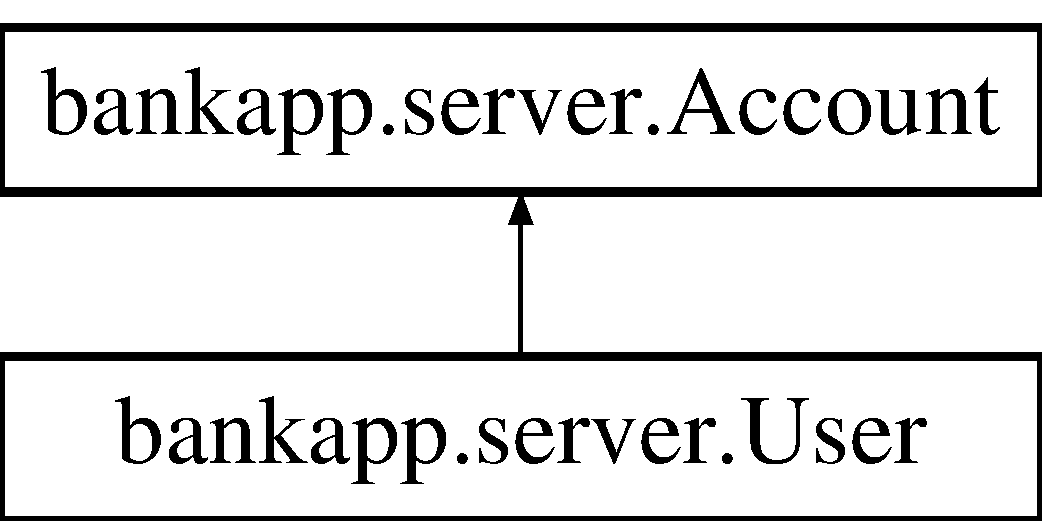
\includegraphics[height=2.000000cm]{classbankapp_1_1server_1_1_user}
\end{center}
\end{figure}
\subsection*{Public Member Functions}
\begin{DoxyCompactItemize}
\item 
\hyperlink{classbankapp_1_1server_1_1_user_ae5d0c0c37ed136f1c3e7534a4af49105}{User} (String username, String pass, String email)
\item 
void \hyperlink{classbankapp_1_1server_1_1_user_a6527a6277676b487137630f595c26248}{deduce\+Account\+Funds} (String acc\+Num, long money)
\item 
void \hyperlink{classbankapp_1_1server_1_1_user_a0da7cce04ab84b5d4ffddeb994516632}{add\+Fundsto\+Account} (String acc\+Num, long money)
\item 
int \hyperlink{classbankapp_1_1server_1_1_user_aa8e72fdac74d28d978bf38711b15dba5}{create\+Account} ()
\item 
void \hyperlink{classbankapp_1_1server_1_1_user_adcf98c41bd09b94a9a068c9bb2fa1f5e}{add\+Account} (\hyperlink{classbankapp_1_1server_1_1bank_account}{bank\+Account} acc)
\item 
String \hyperlink{classbankapp_1_1server_1_1_user_a597376bdfa749415e75185e764b3e04f}{get\+Email} ()
\item 
void \hyperlink{classbankapp_1_1server_1_1_user_aef6765beb0d9556f38070c919ca7e732}{set\+Email} (String email)
\item 
void \hyperlink{classbankapp_1_1server_1_1_user_a90f12d3eae9a484d0f6acc6e74f4a27d}{delete\+Account} (String acc\+Num)
\item 
\hyperlink{classbankapp_1_1server_1_1bank_account}{bank\+Account} \hyperlink{classbankapp_1_1server_1_1_user_a88c5fb41ca03f1b131322ef486fb677d}{get\+Account} (String acc\+Num)
\end{DoxyCompactItemize}


\subsection{Detailed Description}


Definition at line 7 of file User.\+java.



\subsection{Constructor \& Destructor Documentation}
\mbox{\Hypertarget{classbankapp_1_1server_1_1_user_ae5d0c0c37ed136f1c3e7534a4af49105}\label{classbankapp_1_1server_1_1_user_ae5d0c0c37ed136f1c3e7534a4af49105}} 
\index{bankapp\+::server\+::\+User@{bankapp\+::server\+::\+User}!User@{User}}
\index{User@{User}!bankapp\+::server\+::\+User@{bankapp\+::server\+::\+User}}
\subsubsection{\texorpdfstring{User()}{User()}}
{\footnotesize\ttfamily bankapp.\+server.\+User.\+User (\begin{DoxyParamCaption}\item[{String}]{username,  }\item[{String}]{pass,  }\item[{String}]{email }\end{DoxyParamCaption})}



Definition at line 12 of file User.\+java.



\subsection{Member Function Documentation}
\mbox{\Hypertarget{classbankapp_1_1server_1_1_user_adcf98c41bd09b94a9a068c9bb2fa1f5e}\label{classbankapp_1_1server_1_1_user_adcf98c41bd09b94a9a068c9bb2fa1f5e}} 
\index{bankapp\+::server\+::\+User@{bankapp\+::server\+::\+User}!add\+Account@{add\+Account}}
\index{add\+Account@{add\+Account}!bankapp\+::server\+::\+User@{bankapp\+::server\+::\+User}}
\subsubsection{\texorpdfstring{add\+Account()}{addAccount()}}
{\footnotesize\ttfamily void bankapp.\+server.\+User.\+add\+Account (\begin{DoxyParamCaption}\item[{\hyperlink{classbankapp_1_1server_1_1bank_account}{bank\+Account}}]{acc }\end{DoxyParamCaption})}



Definition at line 28 of file User.\+java.

\mbox{\Hypertarget{classbankapp_1_1server_1_1_user_a0da7cce04ab84b5d4ffddeb994516632}\label{classbankapp_1_1server_1_1_user_a0da7cce04ab84b5d4ffddeb994516632}} 
\index{bankapp\+::server\+::\+User@{bankapp\+::server\+::\+User}!add\+Fundsto\+Account@{add\+Fundsto\+Account}}
\index{add\+Fundsto\+Account@{add\+Fundsto\+Account}!bankapp\+::server\+::\+User@{bankapp\+::server\+::\+User}}
\subsubsection{\texorpdfstring{add\+Fundsto\+Account()}{addFundstoAccount()}}
{\footnotesize\ttfamily void bankapp.\+server.\+User.\+add\+Fundsto\+Account (\begin{DoxyParamCaption}\item[{String}]{acc\+Num,  }\item[{long}]{money }\end{DoxyParamCaption})}



Definition at line 20 of file User.\+java.

\mbox{\Hypertarget{classbankapp_1_1server_1_1_user_aa8e72fdac74d28d978bf38711b15dba5}\label{classbankapp_1_1server_1_1_user_aa8e72fdac74d28d978bf38711b15dba5}} 
\index{bankapp\+::server\+::\+User@{bankapp\+::server\+::\+User}!create\+Account@{create\+Account}}
\index{create\+Account@{create\+Account}!bankapp\+::server\+::\+User@{bankapp\+::server\+::\+User}}
\subsubsection{\texorpdfstring{create\+Account()}{createAccount()}}
{\footnotesize\ttfamily int bankapp.\+server.\+User.\+create\+Account (\begin{DoxyParamCaption}{ }\end{DoxyParamCaption})}



Definition at line 23 of file User.\+java.

\mbox{\Hypertarget{classbankapp_1_1server_1_1_user_a6527a6277676b487137630f595c26248}\label{classbankapp_1_1server_1_1_user_a6527a6277676b487137630f595c26248}} 
\index{bankapp\+::server\+::\+User@{bankapp\+::server\+::\+User}!deduce\+Account\+Funds@{deduce\+Account\+Funds}}
\index{deduce\+Account\+Funds@{deduce\+Account\+Funds}!bankapp\+::server\+::\+User@{bankapp\+::server\+::\+User}}
\subsubsection{\texorpdfstring{deduce\+Account\+Funds()}{deduceAccountFunds()}}
{\footnotesize\ttfamily void bankapp.\+server.\+User.\+deduce\+Account\+Funds (\begin{DoxyParamCaption}\item[{String}]{acc\+Num,  }\item[{long}]{money }\end{DoxyParamCaption})}



Definition at line 17 of file User.\+java.

\mbox{\Hypertarget{classbankapp_1_1server_1_1_user_a90f12d3eae9a484d0f6acc6e74f4a27d}\label{classbankapp_1_1server_1_1_user_a90f12d3eae9a484d0f6acc6e74f4a27d}} 
\index{bankapp\+::server\+::\+User@{bankapp\+::server\+::\+User}!delete\+Account@{delete\+Account}}
\index{delete\+Account@{delete\+Account}!bankapp\+::server\+::\+User@{bankapp\+::server\+::\+User}}
\subsubsection{\texorpdfstring{delete\+Account()}{deleteAccount()}}
{\footnotesize\ttfamily void bankapp.\+server.\+User.\+delete\+Account (\begin{DoxyParamCaption}\item[{String}]{acc\+Num }\end{DoxyParamCaption})}



Definition at line 37 of file User.\+java.

\mbox{\Hypertarget{classbankapp_1_1server_1_1_user_a88c5fb41ca03f1b131322ef486fb677d}\label{classbankapp_1_1server_1_1_user_a88c5fb41ca03f1b131322ef486fb677d}} 
\index{bankapp\+::server\+::\+User@{bankapp\+::server\+::\+User}!get\+Account@{get\+Account}}
\index{get\+Account@{get\+Account}!bankapp\+::server\+::\+User@{bankapp\+::server\+::\+User}}
\subsubsection{\texorpdfstring{get\+Account()}{getAccount()}}
{\footnotesize\ttfamily \hyperlink{classbankapp_1_1server_1_1bank_account}{bank\+Account} bankapp.\+server.\+User.\+get\+Account (\begin{DoxyParamCaption}\item[{String}]{acc\+Num }\end{DoxyParamCaption})}



Definition at line 40 of file User.\+java.

\mbox{\Hypertarget{classbankapp_1_1server_1_1_user_a597376bdfa749415e75185e764b3e04f}\label{classbankapp_1_1server_1_1_user_a597376bdfa749415e75185e764b3e04f}} 
\index{bankapp\+::server\+::\+User@{bankapp\+::server\+::\+User}!get\+Email@{get\+Email}}
\index{get\+Email@{get\+Email}!bankapp\+::server\+::\+User@{bankapp\+::server\+::\+User}}
\subsubsection{\texorpdfstring{get\+Email()}{getEmail()}}
{\footnotesize\ttfamily String bankapp.\+server.\+User.\+get\+Email (\begin{DoxyParamCaption}{ }\end{DoxyParamCaption})}



Definition at line 31 of file User.\+java.

\mbox{\Hypertarget{classbankapp_1_1server_1_1_user_aef6765beb0d9556f38070c919ca7e732}\label{classbankapp_1_1server_1_1_user_aef6765beb0d9556f38070c919ca7e732}} 
\index{bankapp\+::server\+::\+User@{bankapp\+::server\+::\+User}!set\+Email@{set\+Email}}
\index{set\+Email@{set\+Email}!bankapp\+::server\+::\+User@{bankapp\+::server\+::\+User}}
\subsubsection{\texorpdfstring{set\+Email()}{setEmail()}}
{\footnotesize\ttfamily void bankapp.\+server.\+User.\+set\+Email (\begin{DoxyParamCaption}\item[{String}]{email }\end{DoxyParamCaption})}



Definition at line 34 of file User.\+java.



The documentation for this class was generated from the following file\+:\begin{DoxyCompactItemize}
\item 
src/main/java/bankapp/server/\hyperlink{_user_8java}{User.\+java}\end{DoxyCompactItemize}

\hypertarget{classbankapp_1_1server_1_1_user_test}{}\section{bankapp.\+server.\+User\+Test Class Reference}
\label{classbankapp_1_1server_1_1_user_test}\index{bankapp.\+server.\+User\+Test@{bankapp.\+server.\+User\+Test}}
\subsection*{Public Member Functions}
\begin{DoxyCompactItemize}
\item 
void \hyperlink{classbankapp_1_1server_1_1_user_test_a81e734600780565479bc7e3e9d58488f}{valid\+User} ()
\item 
void \hyperlink{classbankapp_1_1server_1_1_user_test_aee87b14528a0013dd6fd5ca51c7ec54d}{test\+Add\+Funds} ()
\item 
void \hyperlink{classbankapp_1_1server_1_1_user_test_a5da66e25464ee57cb9e9246c9a026966}{test\+Transaction} ()
\end{DoxyCompactItemize}
\subsection*{Static Protected Attributes}
\begin{DoxyCompactItemize}
\item 
static Validator \hyperlink{classbankapp_1_1server_1_1_user_test_a2cf04df9520daf97f986e1e5d16dcb29}{validator}
\end{DoxyCompactItemize}


\subsection{Detailed Description}


Definition at line 12 of file User\+Test.\+java.



\subsection{Member Function Documentation}
\mbox{\Hypertarget{classbankapp_1_1server_1_1_user_test_aee87b14528a0013dd6fd5ca51c7ec54d}\label{classbankapp_1_1server_1_1_user_test_aee87b14528a0013dd6fd5ca51c7ec54d}} 
\index{bankapp\+::server\+::\+User\+Test@{bankapp\+::server\+::\+User\+Test}!test\+Add\+Funds@{test\+Add\+Funds}}
\index{test\+Add\+Funds@{test\+Add\+Funds}!bankapp\+::server\+::\+User\+Test@{bankapp\+::server\+::\+User\+Test}}
\subsubsection{\texorpdfstring{test\+Add\+Funds()}{testAddFunds()}}
{\footnotesize\ttfamily void bankapp.\+server.\+User\+Test.\+test\+Add\+Funds (\begin{DoxyParamCaption}{ }\end{DoxyParamCaption})}



Definition at line 35 of file User\+Test.\+java.

\mbox{\Hypertarget{classbankapp_1_1server_1_1_user_test_a5da66e25464ee57cb9e9246c9a026966}\label{classbankapp_1_1server_1_1_user_test_a5da66e25464ee57cb9e9246c9a026966}} 
\index{bankapp\+::server\+::\+User\+Test@{bankapp\+::server\+::\+User\+Test}!test\+Transaction@{test\+Transaction}}
\index{test\+Transaction@{test\+Transaction}!bankapp\+::server\+::\+User\+Test@{bankapp\+::server\+::\+User\+Test}}
\subsubsection{\texorpdfstring{test\+Transaction()}{testTransaction()}}
{\footnotesize\ttfamily void bankapp.\+server.\+User\+Test.\+test\+Transaction (\begin{DoxyParamCaption}{ }\end{DoxyParamCaption})}



Definition at line 43 of file User\+Test.\+java.

\mbox{\Hypertarget{classbankapp_1_1server_1_1_user_test_a81e734600780565479bc7e3e9d58488f}\label{classbankapp_1_1server_1_1_user_test_a81e734600780565479bc7e3e9d58488f}} 
\index{bankapp\+::server\+::\+User\+Test@{bankapp\+::server\+::\+User\+Test}!valid\+User@{valid\+User}}
\index{valid\+User@{valid\+User}!bankapp\+::server\+::\+User\+Test@{bankapp\+::server\+::\+User\+Test}}
\subsubsection{\texorpdfstring{valid\+User()}{validUser()}}
{\footnotesize\ttfamily void bankapp.\+server.\+User\+Test.\+valid\+User (\begin{DoxyParamCaption}{ }\end{DoxyParamCaption})}



Definition at line 23 of file User\+Test.\+java.



\subsection{Member Data Documentation}
\mbox{\Hypertarget{classbankapp_1_1server_1_1_user_test_a2cf04df9520daf97f986e1e5d16dcb29}\label{classbankapp_1_1server_1_1_user_test_a2cf04df9520daf97f986e1e5d16dcb29}} 
\index{bankapp\+::server\+::\+User\+Test@{bankapp\+::server\+::\+User\+Test}!validator@{validator}}
\index{validator@{validator}!bankapp\+::server\+::\+User\+Test@{bankapp\+::server\+::\+User\+Test}}
\subsubsection{\texorpdfstring{validator}{validator}}
{\footnotesize\ttfamily Validator bankapp.\+server.\+User\+Test.\+validator\hspace{0.3cm}{\ttfamily [static]}, {\ttfamily [protected]}}



Definition at line 14 of file User\+Test.\+java.



The documentation for this class was generated from the following file\+:\begin{DoxyCompactItemize}
\item 
src/test/java/bankapp/server/\hyperlink{_user_test_8java}{User\+Test.\+java}\end{DoxyCompactItemize}

\chapter{File Documentation}
\hypertarget{_bank_client_8java}{}\section{src/main/java/bankapp/client/\+Bank\+Client.java File Reference}
\label{_bank_client_8java}\index{src/main/java/bankapp/client/\+Bank\+Client.\+java@{src/main/java/bankapp/client/\+Bank\+Client.\+java}}
\subsection*{Classes}
\begin{DoxyCompactItemize}
\item 
class \hyperlink{classbankapp_1_1client_1_1bank_client}{bankapp.\+client.\+bank\+Client}
\end{DoxyCompactItemize}
\subsection*{Packages}
\begin{DoxyCompactItemize}
\item 
package \hyperlink{namespacebankapp_1_1client}{bankapp.\+client}
\end{DoxyCompactItemize}

\hypertarget{_bank_controller_8java}{}\section{src/main/java/bankapp/client/\+Bank\+Controller.java File Reference}
\label{_bank_controller_8java}\index{src/main/java/bankapp/client/\+Bank\+Controller.\+java@{src/main/java/bankapp/client/\+Bank\+Controller.\+java}}
\subsection*{Classes}
\begin{DoxyCompactItemize}
\item 
class \hyperlink{classbankapp_1_1client_1_1bank_controller}{bankapp.\+client.\+bank\+Controller}
\end{DoxyCompactItemize}
\subsection*{Packages}
\begin{DoxyCompactItemize}
\item 
package \hyperlink{namespacebankapp_1_1client}{bankapp.\+client}
\end{DoxyCompactItemize}

\hypertarget{_r_m_i_service_locator_8java}{}\section{src/main/java/bankapp/client/\+R\+M\+I\+Service\+Locator.java File Reference}
\label{_r_m_i_service_locator_8java}\index{src/main/java/bankapp/client/\+R\+M\+I\+Service\+Locator.\+java@{src/main/java/bankapp/client/\+R\+M\+I\+Service\+Locator.\+java}}
\subsection*{Classes}
\begin{DoxyCompactItemize}
\item 
class \hyperlink{classbankapp_1_1client_1_1_r_m_i_service_locator}{bankapp.\+client.\+R\+M\+I\+Service\+Locator}
\end{DoxyCompactItemize}
\subsection*{Packages}
\begin{DoxyCompactItemize}
\item 
package \hyperlink{namespacebankapp_1_1client}{bankapp.\+client}
\end{DoxyCompactItemize}

\hypertarget{_account_8java}{}\section{src/main/java/bankapp/server/\+Account.java File Reference}
\label{_account_8java}\index{src/main/java/bankapp/server/\+Account.\+java@{src/main/java/bankapp/server/\+Account.\+java}}
\subsection*{Classes}
\begin{DoxyCompactItemize}
\item 
class \hyperlink{classbankapp_1_1server_1_1_account}{bankapp.\+server.\+Account}
\end{DoxyCompactItemize}
\subsection*{Packages}
\begin{DoxyCompactItemize}
\item 
package \hyperlink{namespacebankapp_1_1server}{bankapp.\+server}
\end{DoxyCompactItemize}

\hypertarget{_admin_8java}{}\section{src/main/java/bankapp/server/\+Admin.java File Reference}
\label{_admin_8java}\index{src/main/java/bankapp/server/\+Admin.\+java@{src/main/java/bankapp/server/\+Admin.\+java}}
\subsection*{Classes}
\begin{DoxyCompactItemize}
\item 
class \hyperlink{classbankapp_1_1server_1_1_admin}{bankapp.\+server.\+Admin}
\end{DoxyCompactItemize}
\subsection*{Packages}
\begin{DoxyCompactItemize}
\item 
package \hyperlink{namespacebankapp_1_1server}{bankapp.\+server}
\end{DoxyCompactItemize}

\hypertarget{bank_account_8java}{}\section{src/main/java/bankapp/server/bank\+Account.java File Reference}
\label{bank_account_8java}\index{src/main/java/bankapp/server/bank\+Account.\+java@{src/main/java/bankapp/server/bank\+Account.\+java}}
\subsection*{Classes}
\begin{DoxyCompactItemize}
\item 
class \hyperlink{classbankapp_1_1server_1_1bank_account}{bankapp.\+server.\+bank\+Account}
\end{DoxyCompactItemize}
\subsection*{Packages}
\begin{DoxyCompactItemize}
\item 
package \hyperlink{namespacebankapp_1_1server}{bankapp.\+server}
\end{DoxyCompactItemize}

\hypertarget{_bank_d_a_o_8java}{}\section{src/main/java/bankapp/server/\+Bank\+D\+AO.java File Reference}
\label{_bank_d_a_o_8java}\index{src/main/java/bankapp/server/\+Bank\+D\+A\+O.\+java@{src/main/java/bankapp/server/\+Bank\+D\+A\+O.\+java}}
\subsection*{Classes}
\begin{DoxyCompactItemize}
\item 
class \hyperlink{classbankapp_1_1server_1_1bank_d_a_o}{bankapp.\+server.\+bank\+D\+AO}
\end{DoxyCompactItemize}
\subsection*{Packages}
\begin{DoxyCompactItemize}
\item 
package \hyperlink{namespacebankapp_1_1server}{bankapp.\+server}
\end{DoxyCompactItemize}

\hypertarget{_bank_server_8java}{}\section{src/main/java/bankapp/server/\+Bank\+Server.java File Reference}
\label{_bank_server_8java}\index{src/main/java/bankapp/server/\+Bank\+Server.\+java@{src/main/java/bankapp/server/\+Bank\+Server.\+java}}
\subsection*{Classes}
\begin{DoxyCompactItemize}
\item 
class \hyperlink{classbankapp_1_1server_1_1bank_server}{bankapp.\+server.\+bank\+Server}
\end{DoxyCompactItemize}
\subsection*{Packages}
\begin{DoxyCompactItemize}
\item 
package \hyperlink{namespacebankapp_1_1server}{bankapp.\+server}
\end{DoxyCompactItemize}

\hypertarget{_b_manager_8java}{}\section{src/main/java/bankapp/server/\+B\+Manager.java File Reference}
\label{_b_manager_8java}\index{src/main/java/bankapp/server/\+B\+Manager.\+java@{src/main/java/bankapp/server/\+B\+Manager.\+java}}
\subsection*{Classes}
\begin{DoxyCompactItemize}
\item 
class \hyperlink{classbankapp_1_1server_1_1_b_manager}{bankapp.\+server.\+B\+Manager}
\end{DoxyCompactItemize}
\subsection*{Packages}
\begin{DoxyCompactItemize}
\item 
package \hyperlink{namespacebankapp_1_1server}{bankapp.\+server}
\end{DoxyCompactItemize}

\hypertarget{_i_bank_d_a_o_8java}{}\section{src/main/java/bankapp/server/\+I\+Bank\+D\+AO.java File Reference}
\label{_i_bank_d_a_o_8java}\index{src/main/java/bankapp/server/\+I\+Bank\+D\+A\+O.\+java@{src/main/java/bankapp/server/\+I\+Bank\+D\+A\+O.\+java}}
\subsection*{Classes}
\begin{DoxyCompactItemize}
\item 
interface \hyperlink{interfacebankapp_1_1server_1_1_ibank_d_a_o}{bankapp.\+server.\+Ibank\+D\+AO}
\end{DoxyCompactItemize}
\subsection*{Packages}
\begin{DoxyCompactItemize}
\item 
package \hyperlink{namespacebankapp_1_1server}{bankapp.\+server}
\end{DoxyCompactItemize}

\hypertarget{_i_b_manager_8java}{}\section{src/main/java/bankapp/server/\+I\+B\+Manager.java File Reference}
\label{_i_b_manager_8java}\index{src/main/java/bankapp/server/\+I\+B\+Manager.\+java@{src/main/java/bankapp/server/\+I\+B\+Manager.\+java}}
\subsection*{Classes}
\begin{DoxyCompactItemize}
\item 
interface \hyperlink{interfacebankapp_1_1server_1_1_i_b_manager}{bankapp.\+server.\+I\+B\+Manager}
\end{DoxyCompactItemize}
\subsection*{Packages}
\begin{DoxyCompactItemize}
\item 
package \hyperlink{namespacebankapp_1_1server}{bankapp.\+server}
\end{DoxyCompactItemize}

\hypertarget{_report_8java}{}\section{src/main/java/bankapp/server/\+Report.java File Reference}
\label{_report_8java}\index{src/main/java/bankapp/server/\+Report.\+java@{src/main/java/bankapp/server/\+Report.\+java}}
\subsection*{Classes}
\begin{DoxyCompactItemize}
\item 
class \hyperlink{classbankapp_1_1server_1_1_report}{bankapp.\+server.\+Report}
\end{DoxyCompactItemize}
\subsection*{Packages}
\begin{DoxyCompactItemize}
\item 
package \hyperlink{namespacebankapp_1_1server}{bankapp.\+server}
\end{DoxyCompactItemize}

\hypertarget{_user_8java}{}\section{src/main/java/bankapp/server/\+User.java File Reference}
\label{_user_8java}\index{src/main/java/bankapp/server/\+User.\+java@{src/main/java/bankapp/server/\+User.\+java}}
\subsection*{Classes}
\begin{DoxyCompactItemize}
\item 
class \hyperlink{classbankapp_1_1server_1_1_user}{bankapp.\+server.\+User}
\end{DoxyCompactItemize}
\subsection*{Packages}
\begin{DoxyCompactItemize}
\item 
package \hyperlink{namespacebankapp_1_1server}{bankapp.\+server}
\end{DoxyCompactItemize}

\hypertarget{bank_account_test_8java}{}\section{src/test/java/bankapp/server/bank\+Account\+Test.java File Reference}
\label{bank_account_test_8java}\index{src/test/java/bankapp/server/bank\+Account\+Test.\+java@{src/test/java/bankapp/server/bank\+Account\+Test.\+java}}
\subsection*{Classes}
\begin{DoxyCompactItemize}
\item 
class \hyperlink{classbankapp_1_1server_1_1bank_account_test}{bankapp.\+server.\+bank\+Account\+Test}
\end{DoxyCompactItemize}
\subsection*{Packages}
\begin{DoxyCompactItemize}
\item 
package \hyperlink{namespacebankapp_1_1server}{bankapp.\+server}
\end{DoxyCompactItemize}

\hypertarget{_b_d_test_8java}{}\section{src/test/java/bankapp/server/\+B\+D\+Test.java File Reference}
\label{_b_d_test_8java}\index{src/test/java/bankapp/server/\+B\+D\+Test.\+java@{src/test/java/bankapp/server/\+B\+D\+Test.\+java}}
\subsection*{Classes}
\begin{DoxyCompactItemize}
\item 
class \hyperlink{classbankapp_1_1server_1_1_b_d_test}{bankapp.\+server.\+B\+D\+Test}
\end{DoxyCompactItemize}
\subsection*{Packages}
\begin{DoxyCompactItemize}
\item 
package \hyperlink{namespacebankapp_1_1server}{bankapp.\+server}
\end{DoxyCompactItemize}

\hypertarget{_performance_8java}{}\section{src/test/java/bankapp/server/\+Performance.java File Reference}
\label{_performance_8java}\index{src/test/java/bankapp/server/\+Performance.\+java@{src/test/java/bankapp/server/\+Performance.\+java}}
\subsection*{Classes}
\begin{DoxyCompactItemize}
\item 
class \hyperlink{classbankapp_1_1server_1_1_performance}{bankapp.\+server.\+Performance}
\end{DoxyCompactItemize}
\subsection*{Packages}
\begin{DoxyCompactItemize}
\item 
package \hyperlink{namespacebankapp_1_1server}{bankapp.\+server}
\end{DoxyCompactItemize}

\hypertarget{_report_test_8java}{}\section{src/test/java/bankapp/server/\+Report\+Test.java File Reference}
\label{_report_test_8java}\index{src/test/java/bankapp/server/\+Report\+Test.\+java@{src/test/java/bankapp/server/\+Report\+Test.\+java}}
\subsection*{Classes}
\begin{DoxyCompactItemize}
\item 
class \hyperlink{classbankapp_1_1server_1_1_report_test}{bankapp.\+server.\+Report\+Test}
\end{DoxyCompactItemize}
\subsection*{Packages}
\begin{DoxyCompactItemize}
\item 
package \hyperlink{namespacebankapp_1_1server}{bankapp.\+server}
\end{DoxyCompactItemize}

\hypertarget{_server_test_8java}{}\section{src/test/java/bankapp/server/\+Server\+Test.java File Reference}
\label{_server_test_8java}\index{src/test/java/bankapp/server/\+Server\+Test.\+java@{src/test/java/bankapp/server/\+Server\+Test.\+java}}
\subsection*{Classes}
\begin{DoxyCompactItemize}
\item 
class \hyperlink{classbankapp_1_1server_1_1_server_test}{bankapp.\+server.\+Server\+Test}
\end{DoxyCompactItemize}
\subsection*{Packages}
\begin{DoxyCompactItemize}
\item 
package \hyperlink{namespacebankapp_1_1server}{bankapp.\+server}
\end{DoxyCompactItemize}

\hypertarget{_user_test_8java}{}\section{src/test/java/bankapp/server/\+User\+Test.java File Reference}
\label{_user_test_8java}\index{src/test/java/bankapp/server/\+User\+Test.\+java@{src/test/java/bankapp/server/\+User\+Test.\+java}}
\subsection*{Classes}
\begin{DoxyCompactItemize}
\item 
class \hyperlink{classbankapp_1_1server_1_1_user_test}{bankapp.\+server.\+User\+Test}
\end{DoxyCompactItemize}
\subsection*{Packages}
\begin{DoxyCompactItemize}
\item 
package \hyperlink{namespacebankapp_1_1server}{bankapp.\+server}
\end{DoxyCompactItemize}

%--- End generated contents ---

% Index
\backmatter
\newpage
\phantomsection
\clearemptydoublepage
\addcontentsline{toc}{chapter}{Index}
\printindex

\end{document}
